\documentclass[10pt,a4paper]{article}
\usepackage[ngerman]{babel}
\usepackage{graphicx}
\usepackage{float}
\usepackage[labelfont=bf, textfont=it, width= 0.75\textwidth, textformat=period]{caption}
\usepackage[justification=RaggedRight, singlelinecheck=false]{subcaption}
\usepackage{wrapfig}
\usepackage{wallpaper}
\usepackage{booktabs}
\usepackage{amsmath}
\usepackage{esvect}
\usepackage{url}
\usepackage{lmodern}
\usepackage[colorlinks=true,linkcolor=black,urlcolor=cyan,citecolor=black]{hyperref}
\usepackage[left=2.5cm,right=2.5cm,top=2cm,bottom=2cm]{geometry}

%Position des Bildes auf Titelseite
\addtolength{\wpXoffset}{-6,3cm}

\author{Jeremias Beth und Benjamin Lips}
\title{Aerodynamik von Modellraketen: Luftwiderstand und  Flugstabilität}


\begin{document}

\begin{titlepage}
	\centering
	\ThisCenterWallPaper{0.9}{Bilder/FTV-Darstellung.png} %Hintergrundbild von FTV
	{\scshape\huge Gymnasium Eversten Oldenburg} 
	\noindent\rule{\textwidth}{0.5pt} %Horizontale Linie
	{\large \today} %Datum
	\vspace{0.5cm}
	
	
\includegraphics[width=4cm]{Bilder/GEO-logo.png} %Logo der Schule
	
	\vspace{2cm}
	{\LARGE \bfseries Aerodynamik von Modellraketen: %Titel mit richtigem Absatz
	
	\smallskip Luftwiderstand und Flugstabilität}
	
	\vspace{1cm}
	{\large Jeremias Beth und Benjamin Lips} %Autoren
	
	\vspace{3cm}
	{\large Betreut durch: %Betreuer
		
	\smallskip Dr. Ulf Glade}
\end{titlepage}


%Römische Setienzahlen
\pagenumbering{Roman}
\setcounter{page}{2}


\begin{abstract}
	\noindent
	In dieser Arbeit wird der Einfluss der Raketenspitze auf den Flug einer Modellrakete untersucht. Diese Untersuchung findet anhand der selbst gebauten Rakete FTV statt, wobei Luftwiderstand und Flugstabilität untersucht wurden. Es wurden fünf Formen von Raketenspitzen betrachtet.
	
	Die Untersuchung des Luftwiderstandes hat das Ziel, von den Spitzen die mit der grö"sten Flughöhe zu ermitteln. Dafür wird im Windkanal der Widerstandsbeiwert von FTV mit jeder der Spitzen bestimmt. Anschlie"send wird ein möglichst simples Modell entwickelt, mit dem die Flughöhe bestimmt wird. 
	Aus dem Versuch ergab sich, dass die Ogive als Spitzenform im Unterschallbereich den anderen betrachteten Formen in der erreichten theoretischen Flughöhe überlegen war. Die Hypothese, dass ein knickfreier Übergang zwischen Körperrohr und Spitze die Flughöhe verbessert, wurde bestätigt. Die Haack Spitze zeigte allerdings entgegen der Erwartung keine Vorteile.  
	
	Die Untersuchung der Flugstabilität fand zunächst theoretisch statt, wobei ein Verfahren zur Berechnung des Druckpunktes eingesetzt wurde. Zusätzlich wurde ein Versuch im Windkanal durchgeführt.
	Die theoretische Untersuchung ergab, dass FTV mit allen Spitzen ausreichende Flugstabilität aufweist. Diese Ergebnisse konnten durch den Versuch im Windkanal bestätigt werden, wobei zusätzlich festgestellt wurde, dass sich die Rakete quer zum Wind stabil ausrichten kann. Das ist jedoch im Flug sehr unwahrscheinlich.
	
	Im Vergleich der Spitzen lässt sich keine als optimal feststellen. Welche Spitze für eine konkrete Rakete in Bezug auf die Flugstabilität am besten ist, hängt davon ab, ob eine zu gro"se oder kleine Kaliberzahl vorliegt.
\end{abstract}
\newpage


%Inhaltsverzeichnis
\tableofcontents
\newpage



%--------------------------------------------------------------------------------------------------
\section{Einleitung}

%Arabische Seitenzahlen für Hauptteil
\pagenumbering{arabic}
\setcounter{page}{1}

Modellraketen gehören zu den ballistischen Raketen. 
Nach Definition zeichnet ballistische Raketen aus, dass sie nach einer kurzen Beschleunigungsphase einen durch ihre aerodynamischen Eigenschaften bestimmten Kurs verfolgen \cite{brock,hm}. 
Auch wenn der Begriff der ballistischen Rakete leider meist militärisch konnotiert wird, spielen solche Raketen auch in der zivilen Wissenschaft eine Rolle. Aufgrund ihrer gro"sen Flughöhen und ihrer langen Freiflugphase sind sie geeignete Träger für Experimente in der äu"seren Atmosphäre oder in Mirkogravitation \cite{dl}.

Eine besondere Verbreitung genie"sen ballistische Raketen unter nicht-professionellen Anwendern. Die Ursprünge des Amateurraketenbaus gehen zurück in die 1950er Jahre in den USA, wobei es sich dabei zu dieser Zeit um eine sehr gefährliche Freizeitbeschäftigung handelte, da die Raketenantriebe auf abenteuerliche Weise selbst gebaut wurden. Dabei kam es immer wieder zu teilweise schweren Unfällen und Verletzungen. Nach Schätzungen der American Rocket Society wurde in dieser frühen Zeit des Amateurraketenbaus jeder siebte Raketenbauer mindestens einmal verletzt \cite{om,sn}.

Seit 1958 sind fertige Raketenmotoren kommerziell erhältlich, wodurch der gefährlichste Aspekt des Amateurraketenbaus weggefallen ist \cite{sn}. Zusätzlich wurde in den USA 1957 die National Association of Rocketry (NAR) gegründet, welche durch einen Sicherheitskodex die Begriffe Modellrakete und "`High-Power"' Modellrakete (eng. High Power Rocket) definiert. Dieser Kodex findet bis heute weltweit Anerkennung, wodurch der Modellraketenbau im Gegensatz zum frühen Amateurraketenbau zu einem ungefährlichen Hobby geworden ist \cite{om}.

\paragraph{Bedeutung von Aerodynamik}
In der Luft- und Raumfahrt hatte die Aerodynamik schon immer eine gro"se Bedeutung, in den letzten Jahren hat sie sich jedoch in viele neue Gebiete verbreitet. In der Entwicklung von neuen Fortbewegungsmitteln, die möglichst effizient und umweltschonend sind, spielt die Optimierung der Aerodynamik heute eine wichtige Rolle und hat sich somit auf fast alle Bereiche der zivilen Fortbewegung ausgebreitet. Die Methodik dieser Arbeit kann daher nicht nur auf kleine Modellraketen angewendet werden, sondern auch auf die Entwicklung anderer Fahrzeuge.

\paragraph{Eingrenzung des Themas}
Als Versuchsobjekt kommt in dieser Arbeit die selbst entwickelte Modellrakete "`FTV"' (Flight Test Vehicle) zum Einsatz. Somit bezieht sich diese Arbeit auf Geschwindigkeiten im Unterschallbereich.
Untersucht wird der Einfluss der Raketenspitze auf das Flugverhalten. Die Spitze wird direkt von der Luft angeströmt, somit sollte die Raketenspitze einen starken Einfluss auf das Flugverhalten haben. Des Weiteren gibt es bei den Spitzen eine Vielfalt an unterschiedlichen Formen. 

Die Untersuchung findet in zwei gro"sen Themenblöcken statt. Der ersten Block widmet sich dem Einfluss des Luftwiderstandes auf die Flugleistung der Rakete, der zweite Block beschäftigt sich mit der Flugstabilität einer Rakete. Beide Blöcke enthalten experimentelle Anteile, einen Versuch im Windkanal und den Start der Rakete. Die theoretische Untersuchung findet zum Luftwiderstand anhand einer numerischen Flugsimulation statt, zur Untersuchung der Flugstabilität kommt ein analytisches Verfahren zum Einsatz. 

\paragraph{Zielsetzung dieser Arbeit}
Primäres Ziel dieser Arbeit ist es natürlich, einen Einblick in die Auswirkungen der Raketenspitze auf die Flugleistung einer Modellrakete zu erhalten. Darüber hinaus sollen einfache und nachvollziehbare Modelle genutzt bzw. falls mögliche selbst entwickelt werden, um ein besseres Verständnis der zugrunde liegenden Physik zu ermöglichen. Es soll ein breites Spektrum an Methoden eingesetzt werden, sowohl experimentell als auch theoretisch. Um anderen Modellraketenbauern oder Aerodynamikinteressierten unsere Ergebnisse und Methoden zur Verfügung zu stellen, soll das Projekt auf der Plattform  \emph{GitHub} veröffentlicht werden.



%--------------------------------------------------------------------------------------------------
\section{Untersuchungsgegenstand und Versuchsumgebung}

\subsection{Grundlagen des Modellraketenbaus}

Wie bereits erwähnt, wird der Begriff Modellrakete durch einen Sicherheitskodex der NAR definiert. Einige wichtige Punkte sind \cite{om}:
\begin{enumerate}
	\item Modellraketen dürfen nur aus leichten Materialien wie Papier, Holz, Plastik und Gummi hergestellt werden, angepasst an die Motorenstärke und die Leistung der Modellrakete.
	
	\item In Modellraketen dürfen nur geprüfte, industriell gefertigte Raketenmotoren eingesetzt werden. 
	
	\item Es muss ein Bergungssystem verwendet werden, damit die Modellrakete unbeschädigt wieder landen kann und wiederverwendbar ist.
	
	\item Startgewicht und Gesamtimpuls des Motors sind mit $1,5 \text{ kg}$ und $320 \text{ Ns}$ begrenzt.
	
	\item Die Flugstabilität der Rakete ist vor dem ersten Start zu überprüfen.
\end{enumerate}


\subsubsection{Flug einer Modellrakete}
\label{sssec-Flug-einer-Modellrakete}

\begin{wrapfigure}{l}{0.4\textwidth}
	\centering
	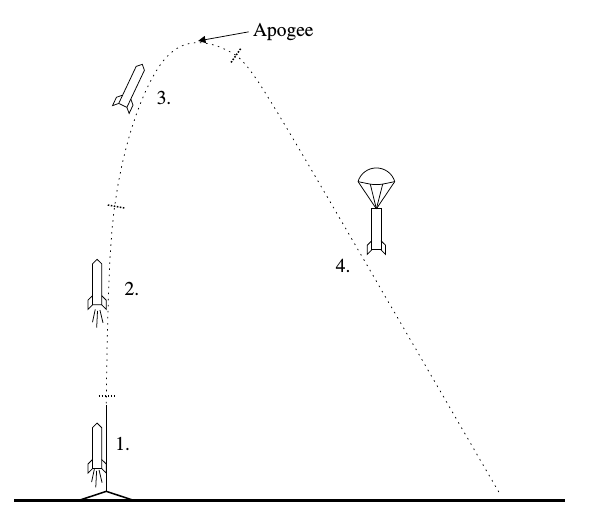
\includegraphics[width=0.3\textwidth]{Bilder/Flug-einer-Modellrakete.png}
	\caption{Die Phasen des Fluges einer Modellrakete \cite{sn}}
	\label{fig-Flug-einer-Modellrakete}
	\vspace{-35pt}
\end{wrapfigure}

Der Flug einer Modellrakete lässt sich durch mehrere Phasen beschreiben \cite{om,sn}:
\begin{enumerate}
	\item \textbf{Start:} Die Rakete hebt ab und verlässt die Startrampe.
	\item \textbf{Beschleunigungsphase:} Durch den Schub des Raketenmotors wird die Rakete beschleunigt.
	\item \textbf{Freiflugphase:} Die Rakete wird in dieser Phase nicht mehr angetrieben, gewinnt aber durch ihre Geschwindigkeit bis zum Erreichen des \textit{Apogäums (eng. Apogee)}, dem höchsten Punkt der Flugbahn, weiter an Höhe.
	\item \textbf{Bergung:} Meist kurz nach dem Apogäum löst das Bergungssystem aus. Die Rakete sinkt dann mit langsamer Geschwindigkeit, bis sie landet.
\end{enumerate}

\noindent
Das "`Timing"' der Flugphasen wird dabei vom Raketenmotor vorgegeben. Siehe \ref{sssec-Aufbau-von-Raketenmotoren} für Näheres.


\subsubsection{Bauteile einer Modellrakete}
\label{sssec-Bauteile-einer-Modellrakete}

Auch wenn es viele unterschiedliche Modellraketen gibt, bleiben noch einige Bauteile, die sich an nahezu jedem Modell finden. Im Folgenden werden die wesentlichen Bauteile einer Modellrakete beschrieben \cite{om}.

\begin{figure}[h]
	\centering
	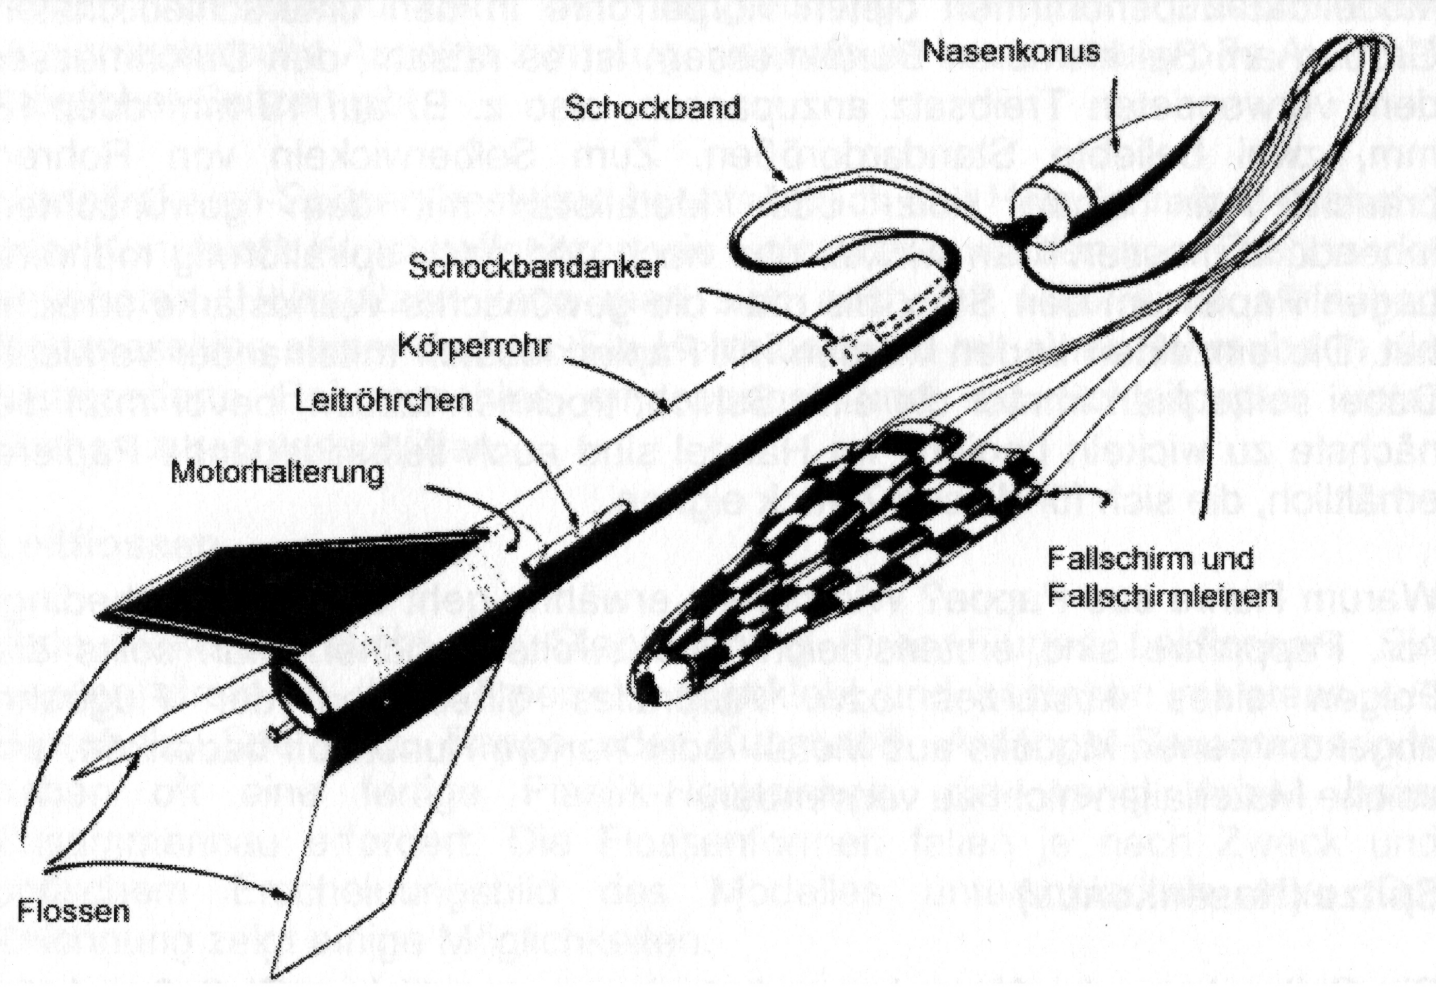
\includegraphics[width=0.5\textwidth]{Bilder/Bauteile-einer-Modellrakete.png}
	\caption{Bauteile einer einfachen Modellrakete \cite{om}}
\end{figure}

\begin{description}
	\item[Körperrohr] Die Funktion des Körperrohrs ist einfach, es stellt den Hauptkörper der Rakete dar.
	
	\item[Flossen bzw. Leitwerke] Diese Bauteile sorgen für die aerodynamische Stabilität der Rakete, da der Flugkörper ansonsten keine senkrechte Flugbahn verfolgen würde \cite{om}.
	
	\item[Nasenkonus] Neben der aerodynamischen Funktion spielt die Spitze auch bei der Bergung der Rakete eine Rolle. Sie wird vom Körperrohr getrennt, um das Bergungssystem freizugeben.
	
	\item[Motorhalterung] Die Motorhalterung bietet eine mechanische Verbindung zwischen dem Raketenmotor und dem Körperrohr.
	
	\item[Bergungssystem] Das Bergungssystem besteht aus einem Fallschirm und dem Schockband, welches diesen mit dem Körperrohr verbindet. Es besteht aus einem elastischen Material, um die kurzzeitig gro"se Kraft beim Öffnen des Fallschirms abzufedern.
	
	\item[Leitröhrchen] Um die Rakete aerodynamisch zu stabilisieren, ist zunächst eine gewisse Geschwindigkeit notwendig. Damit die Rakete zu Beginn des Fluges nicht vom Kurs abweicht, ist sie über die Leitröhrchen mit einer Startvorrichtung verbunden.
\end{description}


\subsubsection{Aufbau von Raketenmotoren}
\label{sssec-Aufbau-von-Raketenmotoren}
 
\begin{figure}[h]
	\centering
	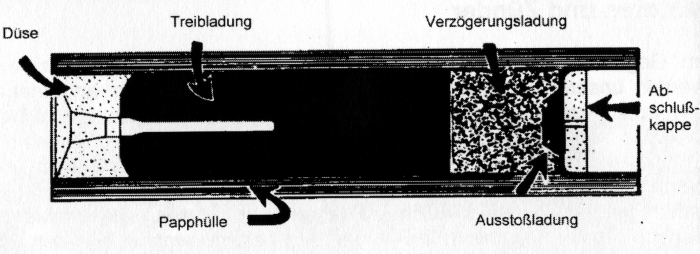
\includegraphics[width=0.5\textwidth]{Bilder/Raketenmotor-Schema.png}
	\caption{Querschnitt eines Raketenmotors \cite{om}}
\end{figure}

\noindent
Alle Raketenmotoren besitzen eine \textit{Treibladung}, welche durch Verbrennung nach dem Rückstoßprinzip eine Schubkraft erzeugt.
Nachdem die Treibladung abgebrannt ist, entzündet sie die \textit{Verzögerungsladung}. Diese ist für die Verzögerungszeit verantwortlich, nach der die \textit{Ausstoßladung} gezündet wird \cite{sn}.
Die Ausstoßladung löst das  Bergungssystems aus, indem sie das Körperrohr unter Druck setzt, und das Bergungssystem herauswirft \cite{om}.

Raketenmotoren werden durch eine Kodierung klassifiziert, wie z.B. \textsf{C6-3}. Der Buchstabe am Anfang gibt einen Bereich für den Gesamtimpuls des Motors in Ns an (siehe Tabelle \ref{tab-Motorkodierungen}).
Die erste Zahl steht für den durchschnittlichen Schub des Raketenmotors in N, wobei der Schub typischerweise meist nicht konstant über die Zeit verläuft, sondern kurz nach der Zündung einen Peak aufweist.
Die letzte Zahl gibt die Verzögerungszeit zwischen Brennschluss und Auslösen der Ausstoßladung an. Bei dem genannten Beispiel \textsf{C6-3} würde es sich also um einen Raketenmotor mit 5 -- 10 Ns Gesamtimpuls handeln, mit einer durchschnittlichen Schubkraft von 6 N und einer Verzögerungszeit von 3 s. 

\begin{table}[H]
\caption{Die Buchstabenkodierungen}
\label{tab-Motorkodierungen}
\centering
\begin{tabular}{r|l}
	\toprule
	Kodierung & Gesamtimpuls [Ns] \\
	\midrule
	A & 1,25 - 2,5 \\
	B & 2,5 - 5 \\
	C & 5 -10 \\
	D & 10 - 20 \\
	E & 20 - 40 \\
	usw. & \dots \\
	\bottomrule
\end{tabular}
\end{table}


\subsection{Der Flugkörper FTV}

Der in diesem Projekt untersuchte Flugkörper \texttt{FTV} besteht aus den in \ref{sssec-Bauteile-einer-Modellrakete} beschriebenen Komponenten einer Modellrakete. Insgesamt weist FTV eine Länge von ca. 68 cm auf, wobei das Körperrohr 50 cm der Länge ausmacht. Die Raketenspitzen haben in etwa eine Länge von 18 cm, wobei es in der Fertigung zu Abweichungen kam. Außerdem besitzt die Rakete drei trapezoide (d.h. trapezförmige) Leitwerke.


\subsubsection{Aufbau}

\begin{figure}[ht]
	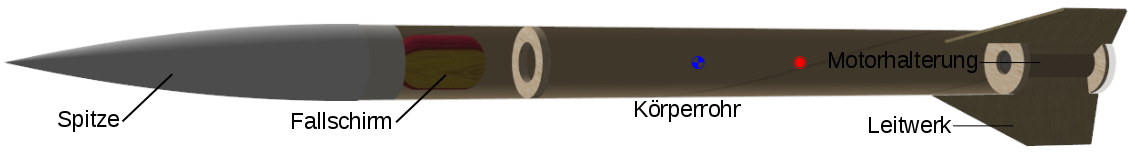
\includegraphics[width=15cm]{Bilder/Bauteile-von-FTV.png}
	\caption{der Flugkörper FTV und seine Bauteile (Screenshot von OpenRocket)}
	\centering
\end{figure}

\begin{description}
	\item[Körperrohr] Bei dem verbautem Körperrohr handelt es sich um ein 40 mm dickes Papprohr, welches im Internetfachhandel für Modellraketenbau erworben wurde.
	
	\item[Motorhalterung] Das Innenrohr der Motorhalterung ist ebenfalls ein Papprohr. Im Gegensatz zu Kunststoffen hält Pappe für die kurze Brenndauer des Raketenmotors die starke Wärmeentwicklung gut aus. Das Innenrohr ist durch Ringe aus Balsaholz im Körperrohr befestigt.
	
	\item[Leitwerke] Als Werkstoff für die Leitwerke wurde 2 mm starkes Balsaholz gewählt. Sie stehen an der breitesten Stelle 32 mm vom Körperrohr ab und reichen durch Schlitze in das Körperrohr hinein.
	
	
	\item[Spitze] Die Raketenspitzen wurden aus dem Kunststoff PLA hergestellt. Um Gewicht einzusparen, sind die Spitzen hohl.
	
	\item[Bergungssystem] Genutzt wird ein Fallschirm mit 50 cm Durchmesser, in Kombination mit einem Schockband aus Elastikband, wie es auch bei Kleidungsstücken zum Einsatz kommt.
\end{description}


\subsubsection{Fertigungsmethoden}
\label{sssec-Fertigungsmethoden}

\paragraph{3D-Druck}
Die Raketenspitzen wurden mit einem handelsüblichen 3D-Drucker hergestellt, mit Schleifpapier nachbearbeitet und anschließend lackiert. Das 3d-Druck-Verfahren bietet eine kostengünstige Methode, um Körper präzise nach einem Modell zu erzeugen. Zwar entstehen durch die Nachbearbeitung Abweichungen, jedoch ist die Oberfläche ohne Bearbeitung zu rau.

\paragraph{CNC-Laserschneider}
Alle Teile aus Balsaholz wurden mit dem Laserschneider des oldenburger Hackspace \emph{Mainframe} aus Platten ausgeschnitten. Dieses Verfahren liefert sehr genaue Ergebnisse.


\subsubsection{Die Raketenspitzen}
\label{sssec-Reketenspitzen}
Für diese Arbeit wurden fünf Raketenspitzen angefertigt, um diese auf ihre aerodynamischen Eigenschaften zu untersuchen. Damit ein Vergleich möglich ist, weisen alle in etwa die selbe Länge auf.
Die Funktion $r(x)$ gibt den Radius der Spitze für jeden Punkt entlang der Mittelachse der Spitze an, wobei die Stelle $x=0$ dem spitzen Ende entspricht. Alle Funktionen $r(x)$ stammen aus \cite{sn}.

\begin{figure}[h]
	\centering
	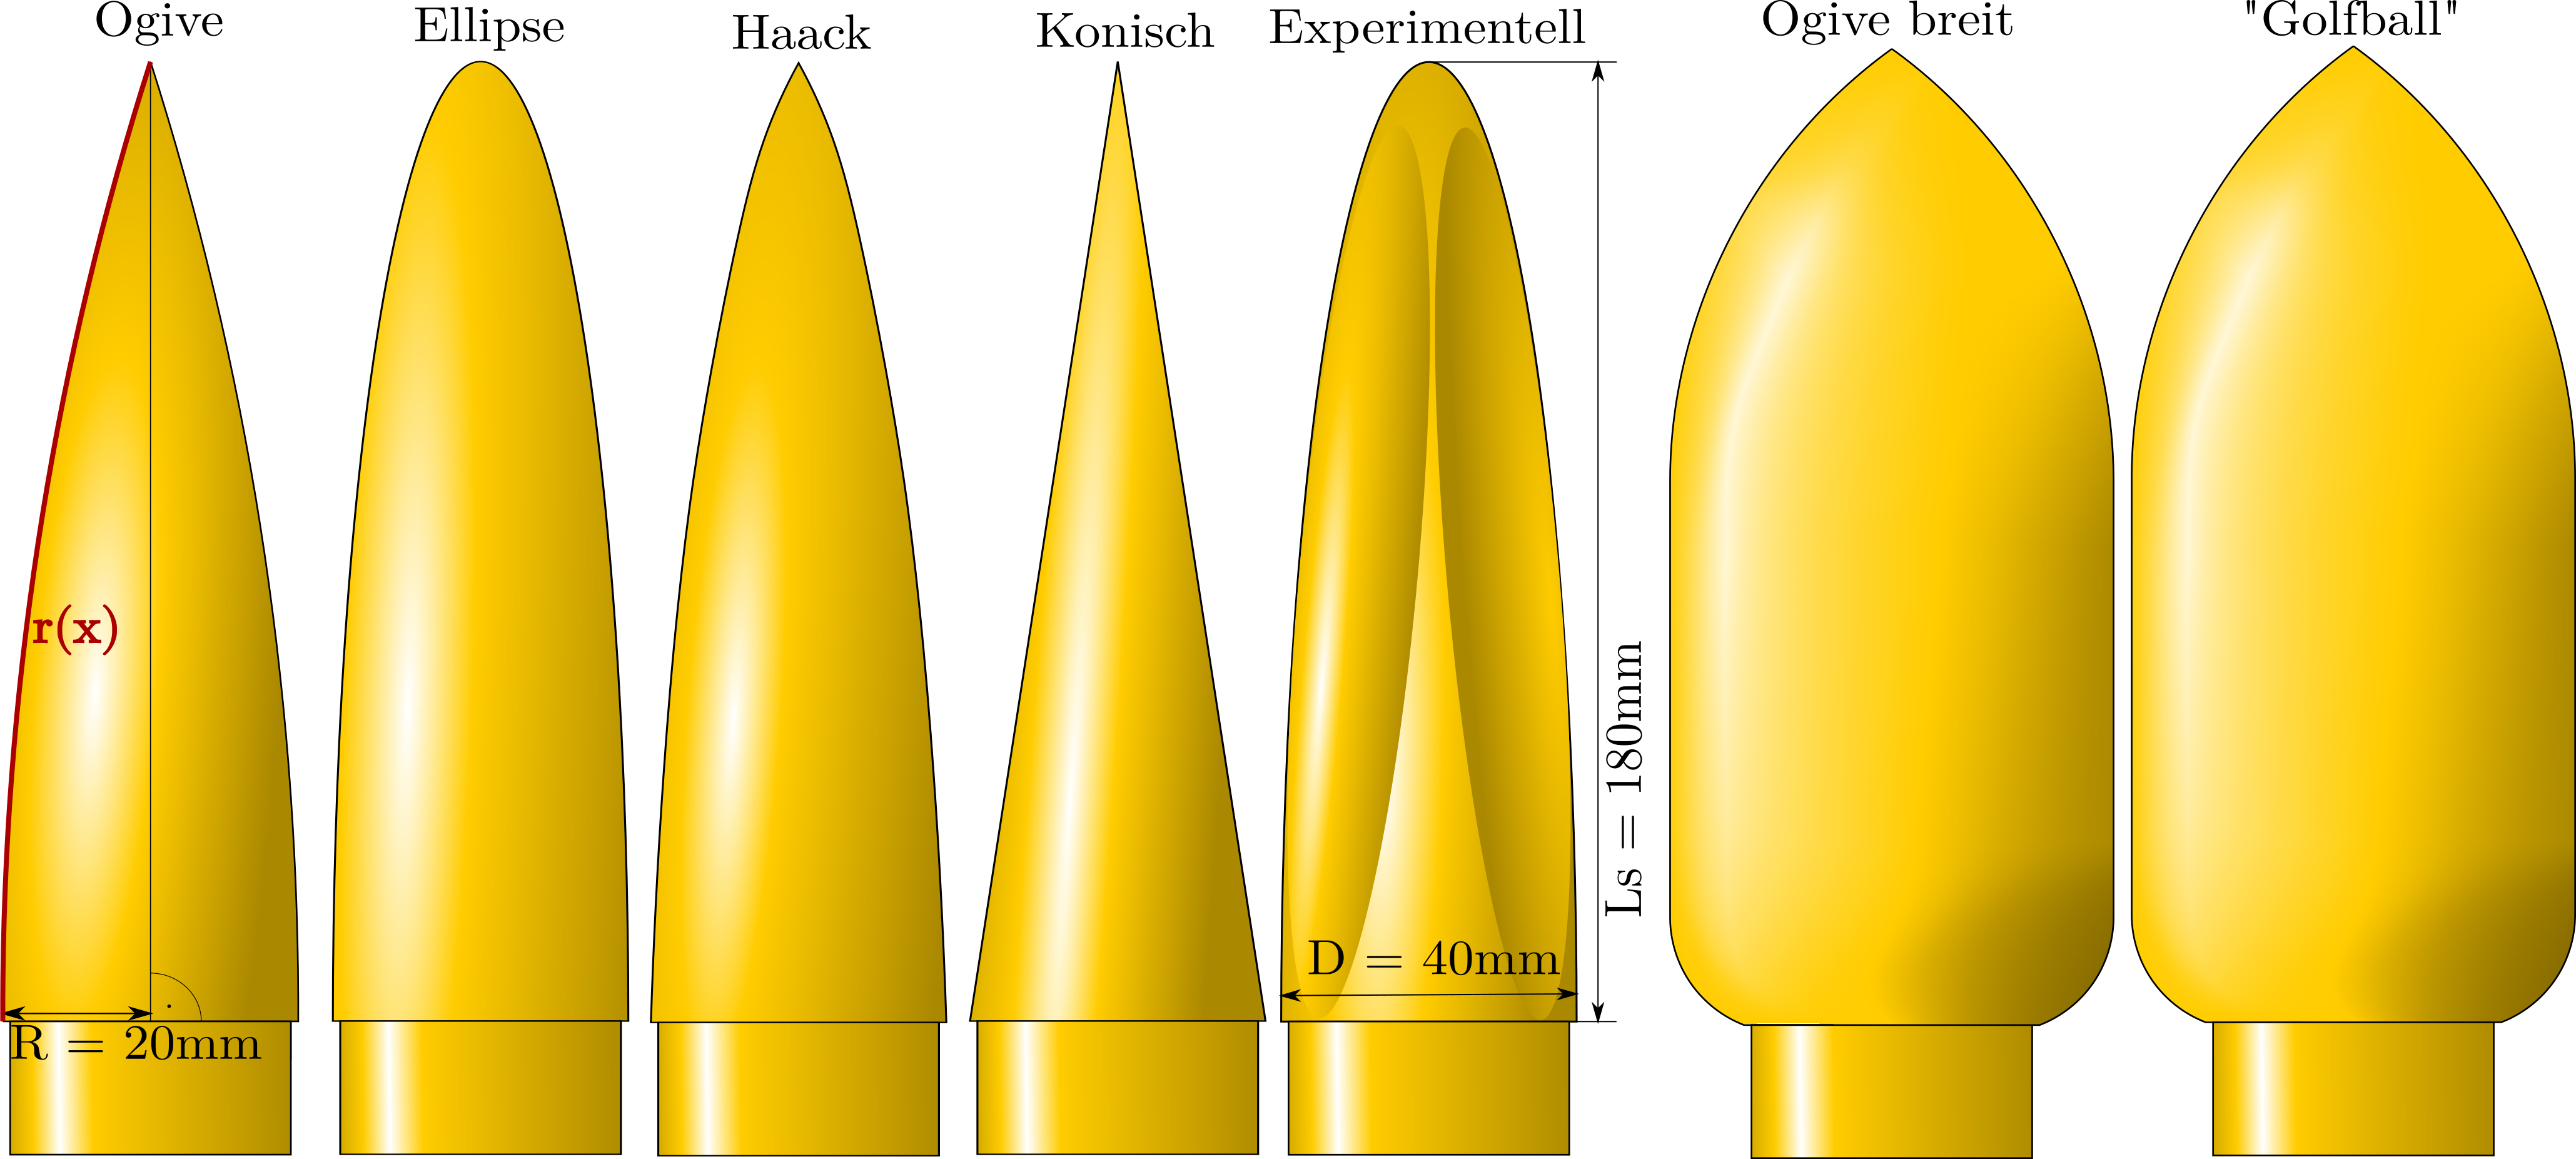
\includegraphics[width=0.6\textwidth]{Bilder/Raketenspitzen.png}
	\caption{Die unterschiedlichen Raketenspitzen (Eigene Grafik)}
	\label{fig-Raketenspitzen}
\end{figure}


\paragraph{Konische Spitze}

Die konische Spitze ist ein Kegel (siehe Abb. \ref{fig-Raketenspitzen}). Dieser ist definiert durch den Radius seiner Basis $R$ und seine Höhe, die der Länge der Spitze $L_{S}$ entspricht.

$$r(x)=\frac{x}{L_{S}} \cdot R \ .$$

\paragraph{Ogive Spitze}
Die Ogive wird durch die Rotation eines Kreisabschnittes geformt. In dieser Arbeit wurde eine tangentiale Ogive betrachtet, d.h. der Übergang zum Körperrohr ist knickfrei (siehe Abb. \ref{fig-Raketenspitzen}).

$$r(x)=\sqrt{\rho_{t}^{2}-(L_{S}-x)^{2}}-\sqrt{\rho_{t}^{2}-L_{S}^{2}} \ \
\text{mit} \ \
\rho_{t}=\frac{R^{2}-L_{S}^{2}}{2 \cdot R} \ .$$ 
  
\noindent
$\rho_{t}$ ist der Radius, welcher die Krümmung des Kreisabschnittes vorgibt.

\paragraph{Elliptische Spitze}
Die elliptische Spitze ist der Rotationskörper einer halben Ellipse mit dem Hauptradius $L_{S}$ und dem Nebenradius $r$ \cite{sn}. So ergibt sich eine komplett knickfreie Spitze (siehe Abb. \ref{fig-Raketenspitzen}).

$$r(x)=R \cdot \sqrt{1-\left( 1-\frac{x}{L_{S}}\right)  ^{2}} \ .$$

\paragraph{Haack Spitze}
In dieser Arbeit wurde eine sog. LV-Haack-Spitze untersucht. Diese liefert eine Form, welche bei konstantem Volumen und konstanter Länge den geringsten Luftwiderstand hat \cite{sn}. Auch wenn sie ursprünglich für den Überschallbereich entwickelt wurde, findet sie manchmal in Modellraketen Verwendung.

$$r(x)=\frac{R}{\sqrt{\pi}} \cdot \sqrt{\varTheta-\tfrac{1}{2} \cdot \sin(2 \cdot \varTheta)+\tfrac{1}{3} \sin^{3} \varTheta} \ \
\text{mit} \ \
\varTheta= \cos^{-1} \left( 1-\frac{2 \cdot x}{L_{S}}\right)  \ .$$

\paragraph{Experimentelle Spitze}
Die experimentelle Spitze ist eine Eigenkreation. Teile ihrer Außenwand sind nach innen geneigt, während andere Abschnitte einer elliptischen Spitze entsprechen. Sie wurde der Untersuchung hinzugefügt, da sie kein Rotationskörper ist (siehe Abb. \ref{fig-Raketenspitzen}).


\subsection{Der Windkanal TWO}

TWO ist einer der Windkanäle der Carl von Ossietzky Universität in Oldenburg.
Der Windkanal ist in der Lage, einen laminaren Luftstrom mit einer Geschwindigkeit von bis zu $20 \text{ ms}^{-1}$ zu produzieren. Der Kanal wird mit einer Spannungsquelle angesteuert, wobei Spannung und Windgeschwindigkeit proportional zueinander sind mit dem Faktor zwei.


\subsection{Verwendete Messinstrumente}

\begin{description}
	\item[Kraftwaage] Der Kraftsensor PCE-FM50 des Herstellers PCE-Instruments hat einen Messbereich von 0~N bis 49 N. Der Sensor hat eine Auflösung von 0,01 N und ist auf $\pm 0,4 \% + 1 \text{ Digit}$ genau \cite{pce}.
	
	\item [Multimeter] Das Digital-Multimeter des Herstellers ELV Elektronik UT~70~A bietet eine Genauigkeit von $\pm0,5 \% + 1 \text{ Digit}$. Genutzt wird es, um Spannungen zu messen \cite{elv}.
\end{description}



%--------------------------------------------------------------------------------------------------
\section{Untersuchung des Luftwiederstandes}

Mit Hilfe von Messwerten soll die ungefähre Flughöhe für jede Spitze ermittelt werden, um einen Vergleichswert zu schaffen. Dazu sollen die in \ref{sssec-Flug-einer-Modellrakete} gezeigten ersten drei Phasen des Fluges untersucht werden. Die Bewegung der Rakete wird dabei vereinfacht als eindimensional in vertikale Richtung dargestellt. 


\subsection{Theoretische Grundlagen}

Die Einflussfaktoren auf den aerodynamischen Widerstand sind anhand einfacher Experimente herleitbar. Hält man während der Fahrt eine Hand aus dem Autofenster, so wird eine spürbare Kraft durch die Luft ausgeübt. Diese Widerstandskraft wirkt auf jeden Körper, der sich durch ein Gas oder eine Flüssigkeit bewegt, da der Körper das Gas um sich verdrängen muss \cite{dlr,lp}. Ziel ist es also, die Spitzenform festzustellen, welche die Luft am effizientesten verdrängt.

Die im Autoexperiment erkennbaren Einflussfaktoren sind die in den Wind gerichtete Fläche, die sich je nach Orientierung der Hand ändert, und die Geschwindigkeit. Ein weiterer Faktor kann in einem weiteren Experiment herausgefunden werden. Bewegt man seine Hand durch Wasser, fällt auf, dass eine größere Kraft aufgebracht werden muss als für die Bewegung durch Luft.

Die Widerstandskraft hängt also von der Querschnittsfläche $A$ des Objekts, seiner Geschwindigkeit $v$ und der Dichte $\rho$ des Mediums ab. Wie Leonardo da Vinci erkannte, wirkt sich allerdings auch die Form des Objektes auf den Luftwiderstand aus \cite{hw}.
Für die vier Einflussfaktoren gilt folgende Gleichung zur Bestimmung der Widerstandskraft $F_{W}$ \cite{lp}:

\begin{equation}
F_{W}=\tfrac{1}{2} A \cdot C_{W} \cdot \rho \cdot v^2
\label{equ-Fw} \ .
\end{equation} 

\noindent
$C_{W}$ ist der sog. Widerstandsbeiwert. Dieser dimensionslose Faktor stellt den Einfluss der Form eines Körpers auf den Luftwiderstand dar. Aus Gleichung \eqref{equ-Fw} geht hervor:

$$ C_{W}=\frac{2 \cdot F_{W}}{\rho \cdot v^2 \cdot A} \ . $$

\noindent
Der $C_{W}$-Wert verhält sich im Bereich unterhalb der Schallgeschwindigkeit nahezu konstant. Die zu erwartenden Geschwindigkeiten von FTV im Flug sind deutlich unterhalb der Schallgeschwindigkeit, somit kann der im Windkanal bei $20 \text{ ms}^{-1}$ bestimmte Wert für $C_{W}$ auf den Flug übertragen werden.


\subsubsection{Bewegung einer Modellrakete} 
Wie in Abb. \ref{fig-Flug-einer-Modellrakete} gezeigt, besteht der Flug einer Modellrakete aus mehreren Abschnitten. Es wirken im Flug drei Kräfte auf die Rakete. Zum einen die beschleunigende Schubkraft $F_{Schub}$ sowie die Gravitationskraft $F_{G}$ und die Luftwiderstandskraft $F_{W}$ in bremsender Wirkung. In der Freiflugphase fällt $F_{Schub}$ weg.

$$ F_{Ges}=F_{Schub}-F_{G}-F_{W} \ . $$

\noindent
$F_{Ges}$ ist die resultierende Kraft, welche auf die Rakete wirkt. Für die Gravitationskraft gilt: $F_{G}=m \cdot g$ \cite{fs}. Eingesetzt ergibt sich für $F_{Ges}$:

$$F_{Ges}=F_{Schub}-m \cdot g-\frac{A \cdot C_{W} \cdot \rho \cdot v^2}{2}  \ . $$

\noindent
Für die Bestimmung der vertikalen Beschleunigung $a$ wird Newton´s zweites Gesetz angewendet. $a$ ist definiert als die ersten Ableitung der Geschwindigkeit $v$:

\begin{equation}
 a(t) = \frac{dv}{dt} = \frac{F_{Schub}}{m}-g-\frac{A \cdot C_{W} \cdot \rho \cdot v(t)^2}{2 \cdot m} \ . 
 \label{equ-Differentialgleichung}
\end{equation}


\subsubsection{Numerische Annäherung an die Flughöhe}\label{sssec-Numerische-Annäherung}
Um die Differenzialgleichung \eqref{equ-Differentialgleichung} zu lösen, wird ein numerisches Verfahren angewendet. Ausgehend vom Startwert $v(0)=0$ wird in sehr kleinen Zeitabständen mit Hilfe der vorherigen Geschwindigkeit $v(t_{n})$ die für den nächsten Zeitpunkt $v(t_{n+1})$ berechnet. Dabei wird angenommen, dass die Widerstandskraft nicht von der aktuellen Geschwindigkeit $v(t_{n+1})$ abhängt, sondern von der vorherigen $v(t_{n})$.

$$ \frac{\Delta v} {\Delta t} = \frac{v(t_{n+1})-v(t_{n})}{t_{n+1}-t_{n}}\approx\frac{F_{Schub}}{m}-g-\frac{A \cdot C_{W} \cdot \rho \cdot v(t_{n})^2}{2 \cdot m} \ . $$

\noindent
Gelöst nach $v(t_{n+1})$:

\begin{equation}
v(t_{n+1})\approx(t_{n+1}-t_{n}) \cdot \left( \frac{F_{Schub}}{m}-g-\frac{A \cdot C_{W} \cdot \rho \cdot v(t_{n})^2}{2 \cdot m} \right) +v(t_{n}) \ .
\end{equation}

\noindent
Durch die Annahme, dass $F_{W}$ von $v(t_{n})$ abhängig ist, entsteht hier eine Ungenauigkeit. Um diese klein zu halten, reicht es nicht, $v$ nur wenige Male für den Flug der Rakete zu berechnen, da $t_{n+1}-t_{n}$ kleinstmöglich gehalten werden soll. Ausgehend von $v$ wird durch Integrieren der zurückgelegte Weg $s$ bestimmt:

$$ s(t) = \int v(t)dt \ . $$


\subsection{Versuch im Windkanal}

\paragraph{Hypothesen}
Da sich ein Ablösen der Strömung von der Spitze negativ auf die Widerstandskraft auswirkt, lassen sich die folgenden Hypothesen aufstellen: \\
Es werden Spitzen mit und ohne knickfreien Übergang zum Körperrohr untersucht. Die Spitzen mit knickfreien Übergängen  sollten weniger Strömungsablösung verursachen als die konischen Spitze ohne. Auch bei der experimentellen Spitze sollte eine größere Ablösung der Strömung der Fall sein. Folglich ist für die konische und experimentelle Spitze ein hoher $C_{W}$-Wert zu erwarten.


\subsubsection{Versuchsaufbau und -durchführung}

Im Versuch wird die Rakete an der Kraftwaage montiert, sodass die Widerstandskraft $F_{W}$ auf die Kraftwaage einwirkt. Die Rakete wird gerade und mittig vor der Öffnung des Windkanals mit der Spitze in den Wind aufgestellt. 

\begin{figure}[H]
	\centering
	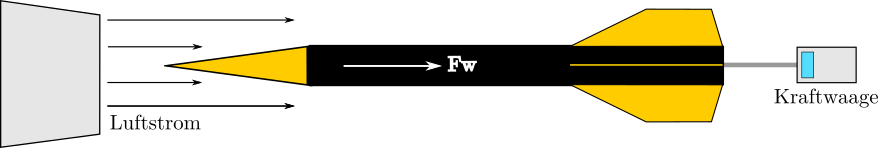
\includegraphics[width=0.6\textwidth]{Bilder/Versuchsaufbau.png}
	\caption{Aufbau des Versuchs (eigene Grafik)}
\end{figure}

\paragraph{Durchführung}
Die Windgeschwindigkeit wird von 0 bis $20 \text{ ms}^{-1}$ erhöht, wobei die Widerstandskraft gemessen wird. Die Daten werden je Spitze zweimal aufgenommen, um Ungenauigkeiten zu verringern.

\paragraph{Methodik der Messwertaufnahme}
Beim Auftragen der gemessenen Kraft gegen die Geschwindigkeit wird bei jeder ersten Änderung der  angezeigten Kraft nach oben die Geschwindigkeit notiert. Schwankt die angezeigte Kraft zwischenzeitlich wieder nach unten, wird dies nicht berücksichtigt. Aus den zwei Messreihen werden nun die durchschnittlichen Geschwindigkeiten bestimmt. Die Windgeschwindigkeit erhält man durch Messen der Steuerspannung.


\subsubsection{Ergebnisse und Auswertung}

\begin{figure}[H]
\begin{subfigure}[l]{0.49\textwidth}
	\centering
	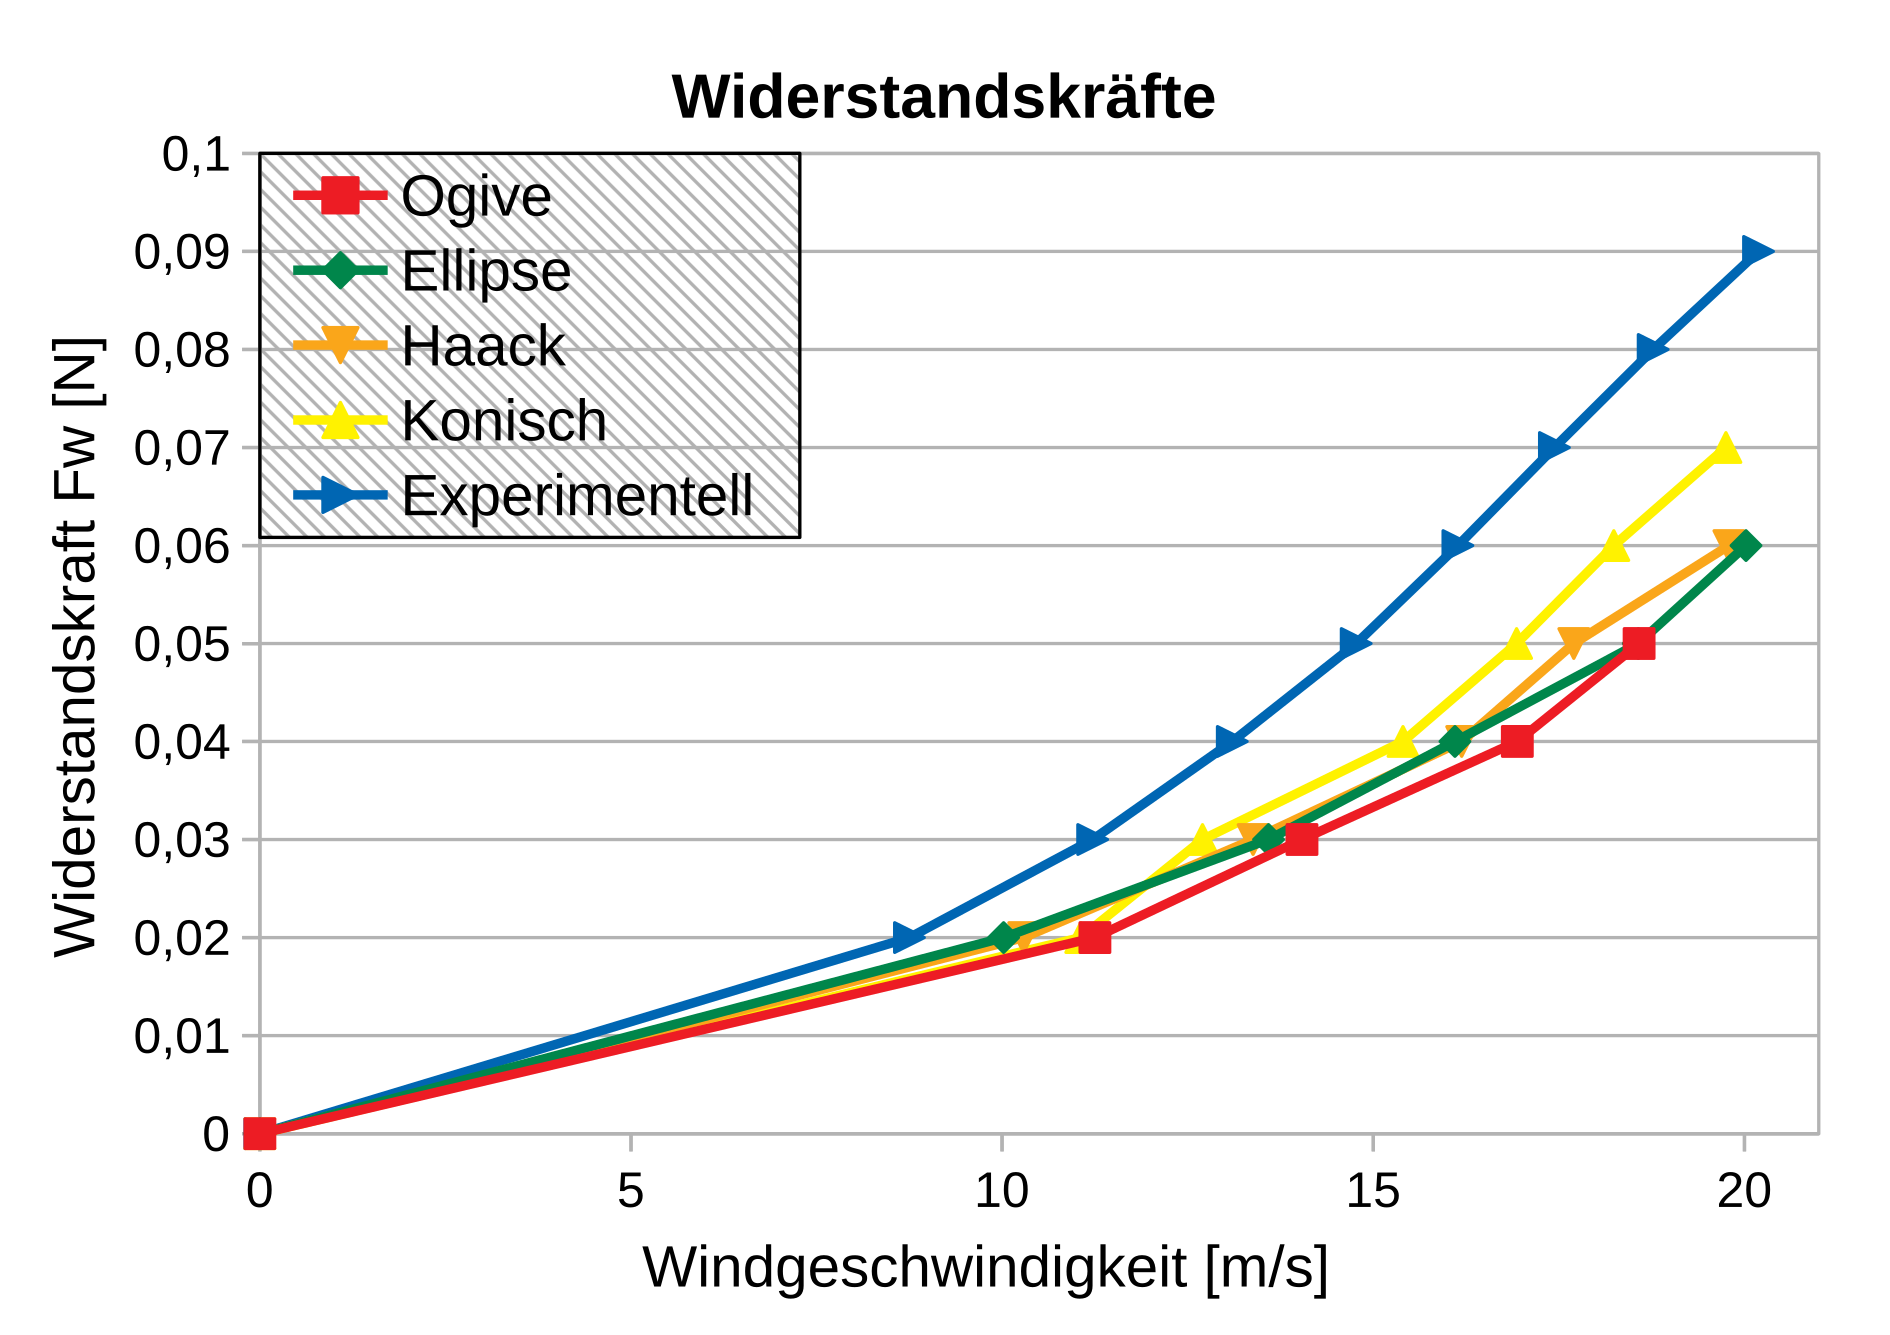
\includegraphics[width=\textwidth]{Bilder/Messwerte-Fw.png}
	\subcaption{Die gemessene Kraft $F_{W}$ aufgetragen über $v$}
	\label{sfig-Messwerte-Fw}
\end{subfigure}
\begin{subfigure}[r]{0.49\textwidth}
	\centering
	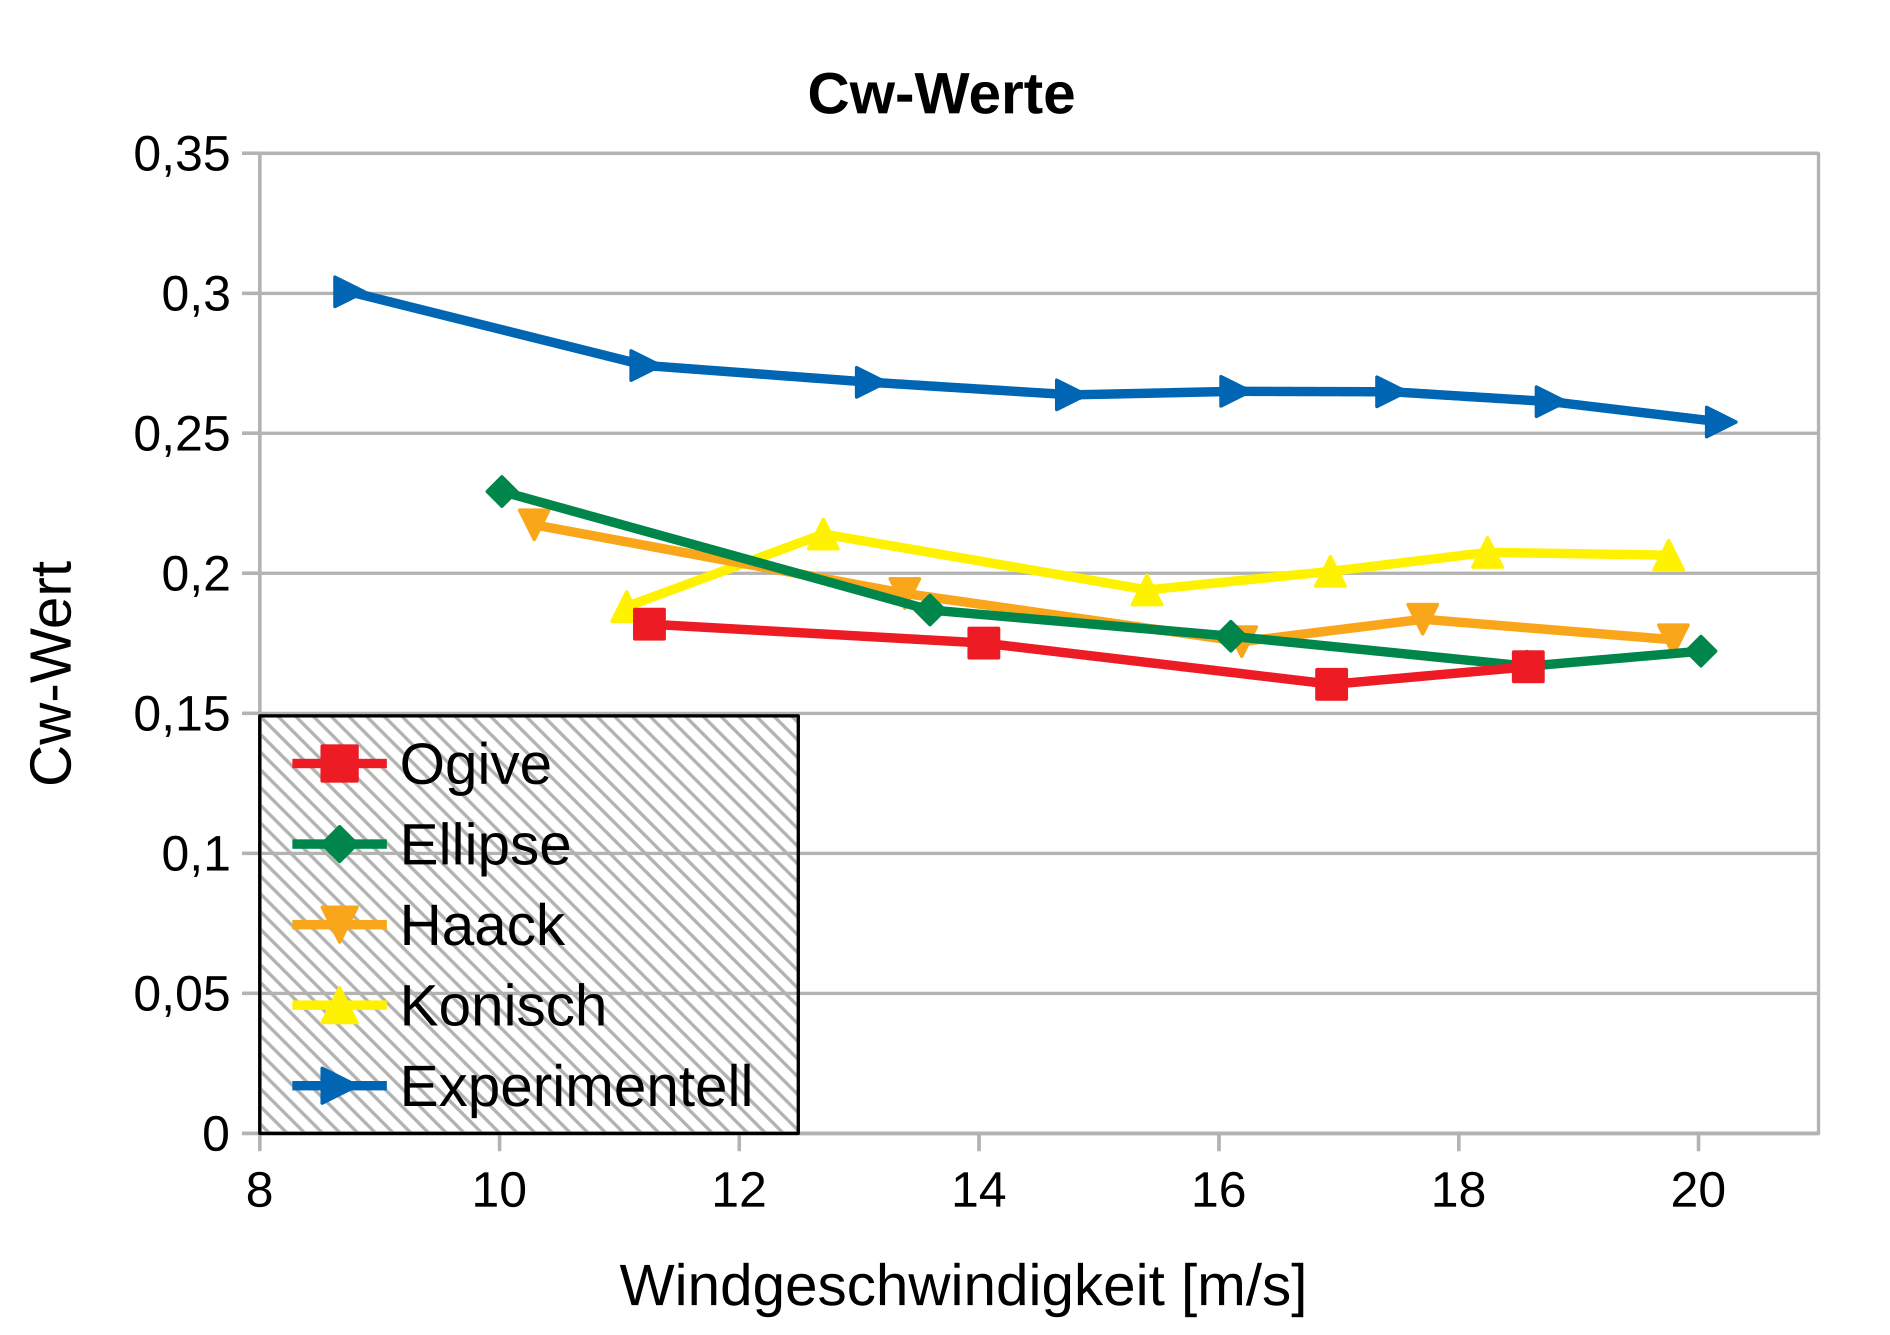
\includegraphics[width=\textwidth]{Bilder/Messwerte-Cw.png}
	\subcaption{Der errechnete $C_{W}$-Wert aufgetragen über $v$}
	\label{sfig-Messwerte-Cw}
\end{subfigure}
\caption{Ergebnisse des Versuches im Windkanal.}
\end{figure}

\paragraph{Gemessene Kräfte}
Das Steigungsverhalten der Kurven gleicht dem einer nach oben geöffneten Parabel (Siehe Abb. \ref{sfig-Messwerte-Fw}). Die geringste gemessene Kraft liegt bei jeder der Spitzen bei 0,02 N. $F_{W}$ ist bei der experimentellen Spitze am größten. Die anderen Graphen liegen nahe beieinander.

\begin{wrapfigure}{r}{0.3\textwidth}
	\vspace{-12pt}
	\centering
	\includegraphics[width=0.3\textwidth]{Bilder/Querschnittsfläche-Rakete.png}
	\caption{die Querschnittsfläche $A$ der Rakete (eigene Grafik)}
	\label{fig-Querschnittsfläche-Rakete}
	\vspace{-20pt}
\end{wrapfigure}

\paragraph{Der errechnete Widerstandsbeiwert}
Zur Berechnung der $C_{W}$-Werte wurde für die Luftdichte ${\rho} = 1,2 \text{ kgm}^{-3}$ angenommen, die Querschnittsfläche der Rakete ergibt sich aus dem Querschnitt der Leitwerke und dem der Spitze (siehe Abb.~\ref{fig-Querschnittsfläche-Rakete}).
So ergeben sich die in Abb. \ref{sfig-Messwerte-Cw} gezeigten $C_{W}$-Werte.

Die errechneten Widerstandsbeiwerte sind nicht konstant. Um einen konstanten Wert zu erhalten, wird aus allen $C_{W}$-Werten einer Spitze der Mittelwert gebildet (Siehe Tabelle \ref{tab-Simulationsparameter} für die $C_{w}$-Werte).

Die Ogive besitzt den kleinsten aerodynamischen Widerstand, gefolgt von Ellipse und Haack-Spitze. Der Wert der konischen Spitze liegt leicht höher, ebenso liegt der der experimentelle Spitze über den der anderen. Somit verursacht die Ogive den geringsten Luftwiderstand. 


\subsection{Flugsimulation}

Das in \ref{sssec-Numerische-Annäherung} beschriebene numerischen Verfahren wurde in der freien Numerik-Software \emph{GNU Octave} umgesetzt. Die Simulation wurde jeweils zweimal durchgeführt, einmal unter Berücksichtigung der Massenunterschiede der Spitzen und einmal mit $m = 0,12 \text{ kg}$, um nur die Spitzenform vergleichen zu können.

\begin{table}[h]
\caption{Parameter für die Flugsimulation}
\begin{subtable}[l]{.49\textwidth}
	\subcaption{Parameter unabhängig der Spitze}
	\begin{tabular}{r|l}
	\toprule
	Parameter	& Wert		\\
	\midrule
	$\rho$ 		& $1,2 \text{ kgm}^{-3}$ \\
	$m$			& $0,12 \text{ kg}$ \\
	$F_{Schub}$	& $9 \text{ N}$ \\
	Schubdauer	& $2,1 \text{ s}$ \\
	$t_{n+1}-t_{n}$ & $10^{-3} \text{ s}$ \\
	\bottomrule
	\end{tabular}
\end{subtable}
\begin{subtable}[l]{.49\textwidth}
	\subcaption{Parameter in Abhängigkeit der Spitze}
	\label{tab-Simulationsparameter}
	\begin{tabular}{r|ll}
	\toprule
	Spitze			& $C_{W}$		& $m$ [kg]	\\
	\midrule
	Ogive			& 0,1710	& 0,118 \\
	Ellipse			& 0,1865	& 0,124 \\
	Haack			& 0,1891	& 0,120 \\
	Konisch			& 0,2016	& 0,114 \\
	Experimentell	& 0,2690	& 0,123 \\
	\bottomrule
	\end{tabular}
\end{subtable}
\end{table}

\begin{figure}
\begin{subfigure}[l]{0.49\textwidth}
	\centering
	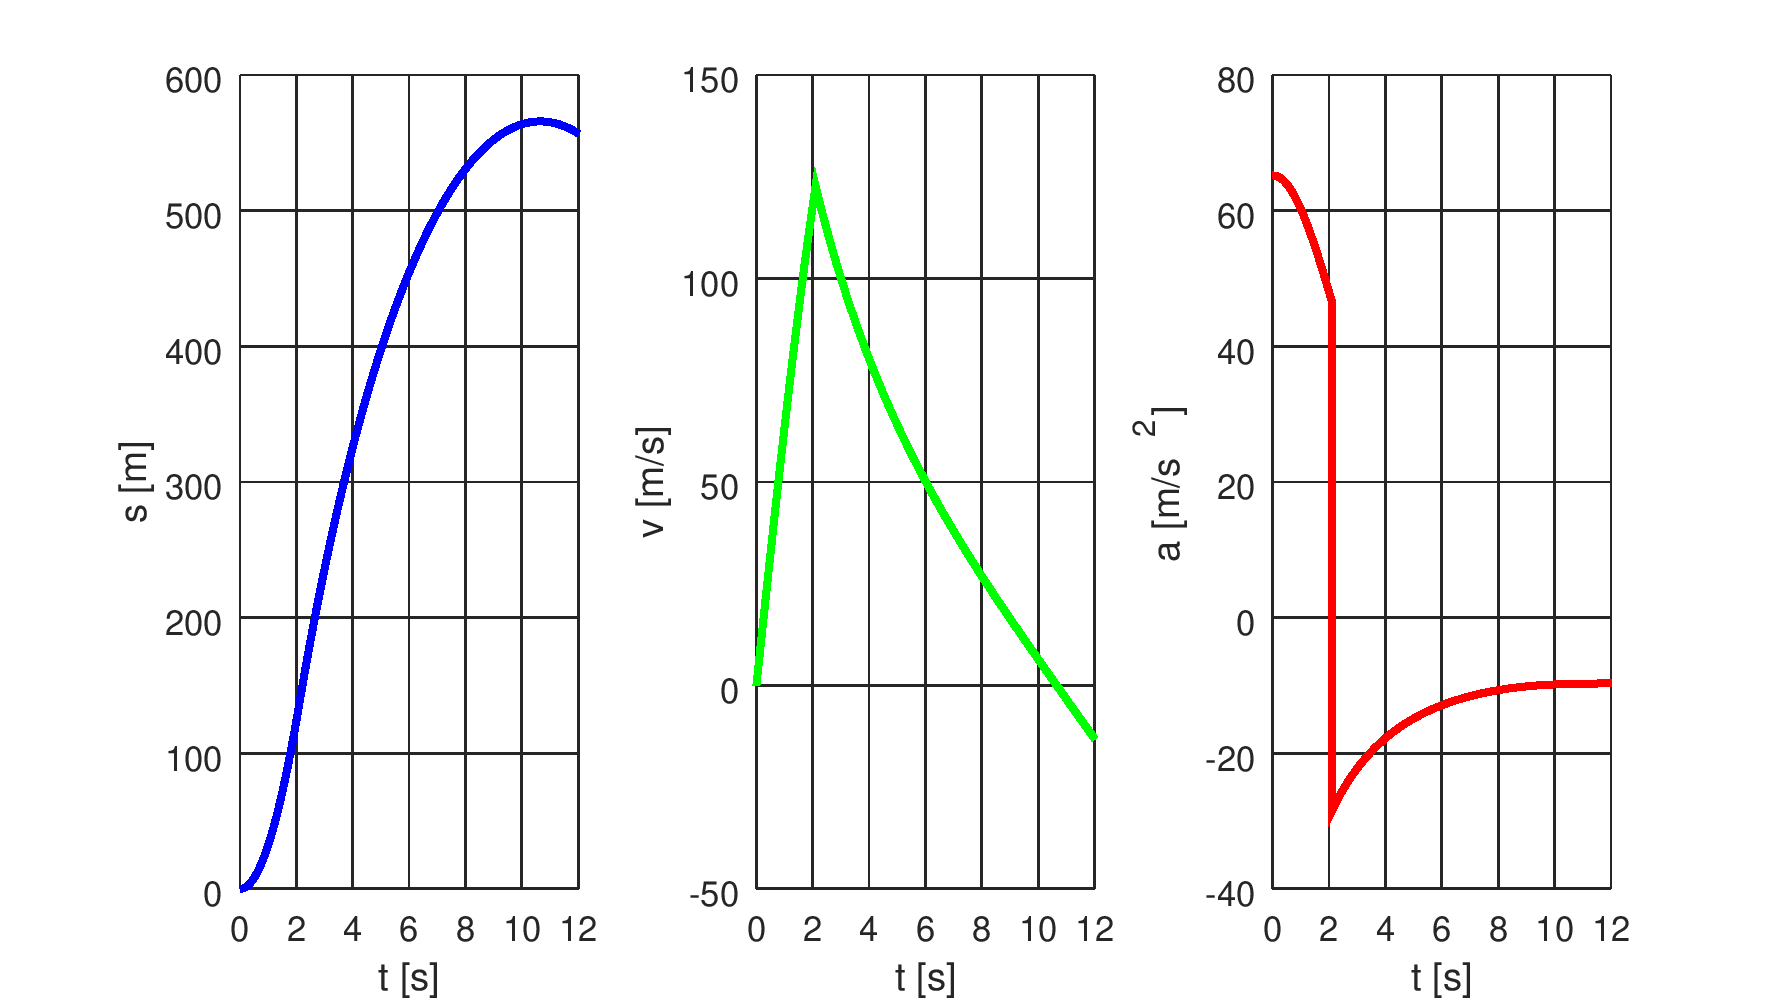
\includegraphics[width=\textwidth]{Bilder/Flugsimulation.png}
	\caption{Flugsimulation von FTV mit ogiver Spitze}
	\label{sfig-Flugsimulation}
\end{subfigure}
\begin{subfigure}[r]{0.49\textwidth}
	\centering
	\includegraphics[width=\textwidth]{Bilder/Simulierte-Flughöhe.png}
	\caption{In der Simulation erreichte Flughöhe}
	\label{sfig-Simulierte-Flughöhe}
\end{subfigure}
\caption{Ergebnisse der Flugsimulation}
\end{figure}

\noindent
Die Ergebnisse in Abb. \ref{sfig-Flugsimulation} geben die Flugphasen einer Modellrakete wieder (siehe \ref{sssec-Flug-einer-Modellrakete}). Bei Betrachtung der Flughöhen mit gleicher angenommener Masse (Abb. \ref{sfig-Simulierte-Flughöhe}) findet sich die selbe Reihenfolge wie bei den $C_{W}$-Werten wieder, die Spitze mit geringstem $C_{W}$ fliegt am höchsten. Unter Berücksichtigung der Masse ändert sich die Reihenfolge, so schneidet die konische Spitze durch ihre geringe Masse besser ab, als die Haack- und elliptische Spitze. Die Ogive schneidet in beiden Fällen am besten ab. Somit ist sie sowohl für die Rakete FTV am besten, als auch ihre Form an sich. 


\subsection{Flugversuch}\label{ssec-Flugversuch-Luftwiderstand}

Der Jungfernflug von FTV fand am 10.01.2019 auf einer großen Wiese in der Nähe von Oldenburg statt, bei fast absoluter Windstille. Zum Einsatz kam ein Raketenmotor vom Typ \textsf{D9-7} und eine Startrampe mit einem ca. $1 \text{ m}$ langen Leitstab.

\paragraph{Ablauf}
Wie erwartet steigt FTV nach dem Start fast senkrecht auf. Kurz nach beenden der Beschleunigungsphase geht der Sichtkontakt zur Rakete verloren, da diese anscheinend in ein Nebelfeld eintritt. Nach mehreren Minuten wird die Suche nach dem Modell begonnen, zunächst jedoch erfolglos. Nach einiger Zeit wird die Spitze der Rakete einzeln wiedergefunden, die Rakete selbst wird erst nach mehr als einer Stunde einige hundert Meter weit vom Startplatz entfernt wiedergefunden. 

\begin{wrapfigure}{r}{0.35\textwidth}
	\vspace{-10pt}
	\includegraphics[width=0.35\textwidth]{Bilder/Höhenmessung.png}
	\caption{Höhenmessung (eigene Abb.)}
	\vspace{-10pt}
\end{wrapfigure}

\paragraph{Beschädigung der Rakete}
Auch wenn das Bergungssystem ausgelöst hat wurden zwei Teile beschädigt: Der Faden zwischen Spitze und Körperrohr ist gerissen und ein Kleinteil der Motorhalterung hat sich gelöst, welches verhindert, dass der Motor hinten aus der Rakete fällt. Dies ist anscheinend passiert, denn der Motor wurde nicht wiedergefunden. 

\paragraph{Höhenmessung}
Die Flughöhe sollte durch Anpeilen der Rakete und eine trigonometrische Berechnung ermittelt werden. Da der Sichtkontakt zur Rakete verloren wurde, konnten leider keine Daten aufgenommen werden. 

\[ h = \tan \alpha \cdot l\]


\subsection{Diskussion}

Da im Flugversuch keine Daten aufgenommen werden konnten, wird für einen realistischen Vergleich die frei Simulations-Software \emph{OpenRocket} eingesetzt. Die Genauigkeit dieser Simulation liegt bei ca. $15 \%$ \cite{sn}. Die Experimentelle Spitze kann mit OpenRocket nicht simuliert werden.

\begin{table}
\caption{Die Eigenen Simulationsergebnisse mit tatsächlicher Masse im Vergleich mit OpenRocket}
\label{tab-Simulationsvergleich}
\centering
\begin{tabular}{r|l|ll}
	\toprule
	\textbf{Spitze} & \multicolumn{3}{c}{\textbf{Erreichte Flughöhe [m]}} \\ \cmidrule{2-4}
	& Eigene Simulation	& OpenRocket	& OpenRocket +15 \%	\\
	\midrule
	Ogive		& 574				& 368			& 423 \\
	Ellipse		& 532				& 357			& 411 \\
	Haack		& 543				& 366			& 421 \\
	Konisch		& 548				& 367			& 422 \\
	\bottomrule
\end{tabular}
\end{table}

In Tabelle \ref{tab-Simulationsvergleich} wird eine deutliche Abweichung zwischen der eigenen Simulation und der durch OpenRocket deutlich. Selbst nach Addition der Ungenauigkeit von OpenRocket fällt die Flughöhe in der eigenen Simulation mit allen Spitzen über $100 \text{ m}$ größer aus. Für diese Abweichungen gibt es verschiedene Gründe. Nicht berücksichtigt wird die Massenabnahme, welche sich durch das Verbrennen der Treibladung ergibt. Außerdem nehmen die Werte von $\rho$ und $F_{G}$ mit größerer Höhe ab, was unser Modell ebenfalls nicht berücksichtigt. Auch für $F_{Schub}$ wurde lediglich der Mittelwert über die Schubdauer eingesetzt.

Der größte Fehler kommt jedoch vermutlich durch die eindimensionale Darstellung zustande. Die Rakete zeigt im Modell immer genau in Flugrichtung. Daher wird an jeder Stelle die kleinstmögliche Widerstandskraft angenommen, was der Theorie nach zu einer maximalen, aber in keiner Weise realistischen Flughöhe führt. 

Des weiteren können auch Messungenauigkeiten als Fehlerquelle eine Rolle spielen. Insbesondere durch die sehr kleinen gemessenen Kräfte sinkt die Genauigkeit der Kraftmessung. Die Fertigung der Spitzen ist auch eine Fehlerquelle, da Abweichungen von der theoretischen Form der Spitzen entstehen (siehe \ref{sssec-Fertigungsmethoden}).



%--------------------------------------------------------------------------------------------------
\section{Untersuchung der Flugstabilität}

Damit Raketen auf ihrer Flugbahn bleiben, müssen sie stabilisiert werden \cite{dl}. Bei FTV handelt es sich wie bei nahezu allen Modellraketen um eine aerodynamisch stabilisierte Rakete.


\subsection{Theoretische Betrachtung der Flugstabilität}
\label{ssec-Theoretische-Btrachtung-Flugstabilität}

\paragraph{Bewegungsrichtungen}

\begin{figure}[h]
\begin{subfigure}[l]{0.49\textwidth}
	\centering
	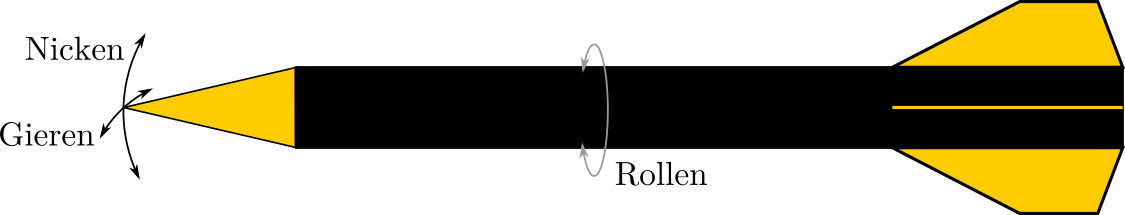
\includegraphics[width=\textwidth]{Bilder/Freiheitsgrade.png}
	\subcaption{Die Freiheitsgrade der Drehbewegung einer Rakete (eigene Grafik)}
	\label{sfig-Freihetsgrade}
\end{subfigure}
\begin{subfigure}[l]{0.49\textwidth}
	\centering
	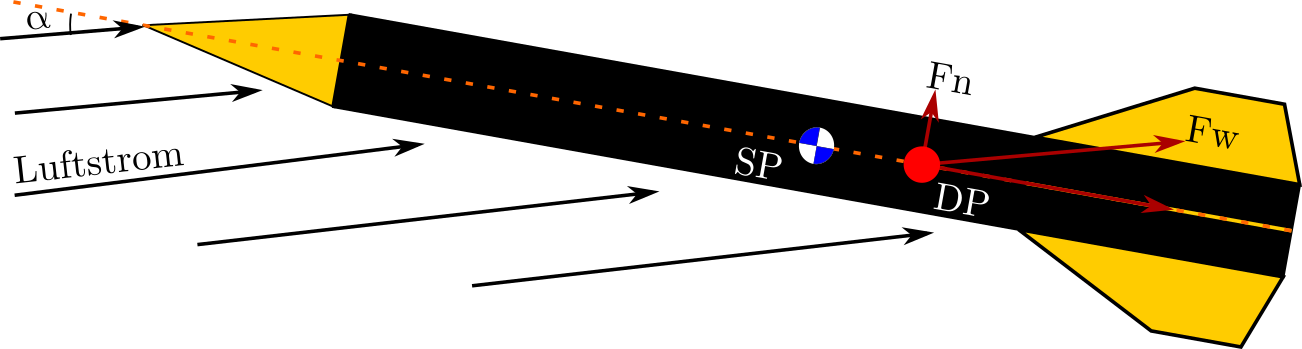
\includegraphics[width=\textwidth]{Bilder/Lage-DP-SP.png}
	\caption{Die Lage von SP und DP (eigene Grafik)}
	\label{sfig-Lage-DP-SP}
\end{subfigure}
\caption{Drehbewegung einer Modellrakete}
\end{figure}

Die Drehbewegung einer Rakete kann in Nicken, Gieren und Rollen eingeteilt werden. Dabei heißt die Bewegung um die Längsachse Rollen, die Nick- und Gierachse sind orthogonal zur Längsachse und zueinander (siehe Abb. \ref{sfig-Freihetsgrade}). Eine Unterscheidung zwischen Nicken und Gieren ist bei Raketen schwierig, da es keine geometrischen Unterschiede zwischen Nicken und Gieren gibt \cite{AbR}.

\paragraph{Stabilisierung der Bewegung}
Damit eine Rakete möglichst hoch fliegt und keine Gefahr für Personen darstellt, sollte sie senkrecht hoch fliegen. Um dies zu erreichen, muss die Bewegung der Rakete stabilisiert werden, wobei die Rollbewegung irrelevant ist.

Die Stabilität der Rakete hängt von der Lage des \textit{Schwerpunktes} (SP) und des \textit{Druckpunktes} (DP) ab (siehe Abb. \ref{sfig-Lage-DP-SP}) \cite{AbR}. Der Schwerpunkt ist der  Drehpunkt der Rakete, im Druckpunkt setzt die aerodynamische Widerstandskraft $ \vv{F_{W}} $ \cite{AbR} an.
Damit eine Rakete aerodynamisch stabil ist, muss der Druckpunkt hinter dem Schwerpunkt liegen \cite{AbR,om}. Wenn die Rakete von ihrem Kurs abweicht, dann ist der \textit{Angriffswinkel} $\alpha \neq 0$. Das liegt an der Trägheit der Rakete, sie dreht sich, die Flugrichtung folgt erst später. Die Widerstandskraft $\vv{F_{W}}$ besitzt eine Komponenten $F_{n}$, die senkrecht zur Längsachse ist und ein Drehmoment auf die Rakete ausübt. Liegt der DP hinter dem SP, dann korrigiert dieses Drehmoment die Schieflage der Rakete.
Als Maß der Stabilität einer Rakete wird häufig die sog. \textit{Kaliberzahl} \texttt{Kal} herangezogen \cite{AbR,dl,om,sn}. Diese gibt den Abstand zwischen DP und SP als Vielfaches des Raketendurchmessers $D$ an:
\begin{equation}
\mathtt{Kal} = \frac{x_{SP}-x_{DP}}{D} \ .
\end{equation}

\noindent
Dabei sind $x_{SP}$ und $x_{DP}$ die Strecken von der Unterkante der Rakete zum SP bzw. DP. Liegt \texttt{Kal} zwischen $1$ und $2,5$, kann ein stabiles Flugverhalten angenommen werden. Ist der Wert zu klein oder zu groß, dann ist die Rakete nicht ausreichend stabil oder reagiert zu stark auf äußere Störungen \cite{om}.

Um vorauszusagen, ob eine Rakete stabil fliegt oder nicht, muss die Lage beider Punkte bekannt sein. Während sich die Position des SP leicht experimentell bestimmen lässt, ist die Position des DP nur schwierig durch einen Versuch festzustellen. Deshalb soll die Lage vom DP theoretisch bestimmt werden.


\subsubsection{Theoretische Vorhersage des Druckpunktes}

\label{Theorie-Stabi-Sec}
Bei der hier beschriebenen Methode zur Berechnung des DP handelt es sich um eine vereinfachte Variante der in \cite{sn} beschriebenen Methode. Dementsprechend stammen auch die folgenden Gleichungen aus \cite{sn}, mit Ausnahme von Gleichung \eqref{equ-Gamma-Vollständig}, welche selbst hergeleitet wurde.
\medskip

\noindent
Voraussetzung für die theoretische Vorhersage des DP sind \cite{sn}:
\begin{enumerate}
	\item Der Angriffswinkel $ \alpha $ (siehe Abb. \ref{sfig-Lage-DP-SP}) ist nahe Null.
	\item Der Luftstrom um die Rakete ist laminar.
	\item Die Raketenspitze läuft spitz zu.
	\item Die Leitwerke sind flach.
	\item Die Rakete ist achsensymmetrisch.
\end{enumerate}

\noindent
Nehmen wir an, dass die Rakete an dem Punkt $X_{0}$ an ihrem unteren Ende der Rakete auf der Längsachse fixiert ist, dann ruft die Auftriebskraft $F_{n}$ ein Drehmoment $M_{n}$ um $X_{0}$ hervor, für welches gilt:

\[ M_{n} = F_{n} \cdot x_{DP} \]
\[ \Rightarrow x_{DP} = \frac{F_{n} \cdot x_{DP}}  {F_{n}} \ . \]

\noindent
Da es schwierig ist mit $F_{n}$ zu hantieren \cite{sn}, kommt stattdessen der \textit{Auftriebsbeiwert} $C_{n}$ zum Einsatz:

\[ C_{n} = \dfrac{F_{n}}{\tfrac{1}{2} \cdot \rho \cdot v^{2} \cdot A_{ref}} \ . \]

\noindent
$A_{ref}$ ist dabei eine Referenzfläche, für die genau genommen ein beliebiger Wert eingesetzt werden kann, ohne dass es für das Ergebnis von $x_{DP}$ einen Unterschied macht. Der Wert ist trotzdem notwendig, da $C_{n}$ ansonsten nicht einheitenlos wäre \cite{sn}.
Durch Einsetzen kann $x_{DP}$ folglich auch durch

\[ x_{DP} = \frac{C_{n} \cdot x_{DP}}{C_{n}}  \]

\noindent
beschrieben werden. Da es schwierig ist, den Auftriebsbeiwert des gesamten Flugkörpers zu bestimmen, werden die Bauteile der Rakete zunächst einzeln betrachtet. Danach kann $x_{DP}$  berechnet werden \cite{AbR,sn},

\[ x_{DP} = \sum_{i=1}^{n} \frac{C_{n_{i}} \cdot x_{i}} {C_{n_{i}}}  \]

\noindent
wobei $C_{n_{i}}$ die Auftriebsbeiwerte der einzelnen Bauteile sind und $x_{i}$ die Strecken von den Druckpunkten der einzelnen Bauteile zu $X_{0}$.

Die Bauteile, die einen Einfluss auf $x_{DP}$ haben, sind die Spitze, das Körperrohr und die Leitwerke. Alle anderen Bauteile werden nicht vom Luftstrom getroffen. Der Einfluss des Körperrohres ist so gering, dass er vernachlässigt werden kann, weil bei kleinen Angriffswinkeln $\alpha$ fast gar keine Fläche zum Luftstrom zeigt \cite{AbR}. Somit bleiben nur noch die Parameter $C_{n_{S}}$ und $x_{S}$ für die Raketenspitze und $C_{n_{LL}}$ und $x_{LL}$ für die Leitwerke:

\begin{equation}
x_{DP} = \frac{C_{n_{S}} \cdot x_{S} + C_{n_{LL}} \cdot x_{LL}} {C_{n_{S}} + C_{n_{LL}}} \ .
\end{equation}

\paragraph{Die Werte $C_{n_{S}}$ und $x_{S}$ für die Spitzen} 
Für $C_{n_{S}}$ gilt:

\begin{equation}
C_{n_{S}} = \frac{2}{A_{ref}} \cdot A_{S} \ .
\label{equ-Cn_S}
\end{equation}

\noindent
Dabei ist $A_{S}$ die Querschnittfläche der Spitze an ihrer Basis. Die Position des DP von der Spitze $x_{S}$ berechnet sich nach

\begin{equation}
x_{S} = L_{S} - \frac{L_{S} \cdot A_{S} - V_{S}}{A_{S}} + L_{K} \ ,
\end{equation}

\noindent
mit der Länge $L_{S}$ und dem Volumen $V_{S}$ der Spitze. Die Länge des Körperrohrs $L_{K}$ wird addiert, da $x_{S}$ die Strecke von der Unterkante der gesamten Rakete zum DP der Spitze ist.
Abgesehen von der experimentelle Spitze handelt es sich bei den untersuchten Spitzen um Rotationskörper. Ihr Volumen wird durch Integrieren der Funktion $r(x)$ bestimmt (siehe \ref{sssec-Reketenspitzen}):

\[ V_{S} = \pi \cdot \int_{0}^{L_{S}}[r(x)]^{2} \mathrm{d}x \ .\]

\noindent
Das Volumen unserer experimentellen Spitze lässt sich nur schwer in eine Formel fassen. Deshalb wird ihr Volumen durch die CAD-Software \emph{Autodesk Fusion 360\texttrademark} berechnet.

\paragraph{Die Werte $C_{n_{LL}}$ und $x_{LL}$ für die Leitwerke}

\begin{figure}[H]
	\centering
	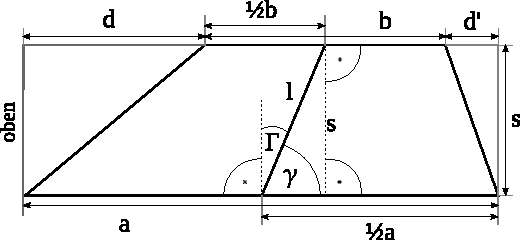
\includegraphics[width=0.4\textwidth]{Bilder/Leitwerk-Geometrie.pdf}
	\caption{Die Geometrie eines trapezoiden Leitwerks (eigene Grafik)}
	\label{Leitwerk-Geometrie-Abb}
\end{figure}

Der Auftriebsbeiwert $C_{n_{LL}}$ von $n$ Leitwerken berechnet sich durch \cite{sn}
\[ C_{n_{LL}} = \frac{n}{2} \cdot C_{n_{L}} \cdot K \ .\]

\noindent
$K$ ist ein Korrekturfaktor, welcher die Interferenz zwischen Leitwerken und Körperrohr berücksichtigt, $C_{n_{L}}$ ist der Auftriebsbeiwert eines Leitwerkes.
Mit $K=1+\frac{D}{2s + D}$ \cite{AbR,sn}, wobei $D$ der Durchmesser der Rakete ist und $s$ die Höhe der Leitwerke (siehe Abb. \ref{Leitwerk-Geometrie-Abb}), ergibt sich:

\begin{equation}
C_{n_{LL}} = \frac{n}{2} \cdot C_{n_{L}} \cdot \left(1+\frac{D}{2s + D}\right) \ .
\end{equation}

\noindent
Für $C_{n_{L}}$ gilt für Geschwindigkeiten weit unterhalb der Schallgeschwindigkeit \cite{sn}:

\begin{equation}
C_{n_{L}} = \dfrac{2\pi \cdot \frac{s^{2}}{A_{ref}}} {1+ \sqrt{1+ \left(\frac{s^{2}}{A_{L} \cdot \cos \Gamma}\right) ^{2} }} \ .
\end{equation}

\noindent
Dabei ist ${A_{L}}$ die Fläche eines Leitwerkes. 
Für $\Gamma$ gilt (siehe Abb. \ref{Leitwerk-Geometrie-Abb}):

\begin{equation}
\Gamma = \tfrac{1}{2} \pi - \gamma \ .
\label{equ-Gamma}
\end{equation}

\noindent
$\gamma$ kann dargestellt werden als:

\[ \gamma = \arccos \frac{\tfrac{1}{2}a - \left(\tfrac{1}{2}b + d'\right) }{l} \ .\]

\noindent
Aus dem Satz des Pythagoras ergibt sich für $l$:

\[ l = \sqrt{\left(\tfrac{1}{2}a-\tfrac{1}{2}b-d'\right) ^{2}+s^{2}} \ .\]

\noindent
Einsetzen in \eqref{equ-Gamma} liefert:

\begin{equation}
\Gamma = \tfrac{1}{2}\pi - \arccos \dfrac{\tfrac{1}{2}a - \tfrac{1}{2}b - d' }   {\sqrt{\left(\tfrac{1}{2}a-\tfrac{1}{2}b-d'\right) ^{2}+s^{2}}} \ .
\label{equ-Gamma-Vollständig}
\end{equation}

\noindent
Für $x_{LL}$ gilt \cite{sn}:

\begin{equation}
x_{LL} = a - \frac{d}{3} \cdot \frac{a+2b}{a+b} - \frac{1}{6} \cdot \frac{a^{2}+b^{2}+ab} {a+b} \ .
\end{equation}


\subsubsection{Betrachtung der Stabilität von FTV}

Wie in \ref{ssec-Theoretische-Btrachtung-Flugstabilität} erwähnt, muss für die Beurteilung der aerodynamischen Stabilität einer Rakete zunächst Druck- und Schwerpunkt bekannt sein.

\paragraph{Vorhersage des Druckpunktes}
Hier soll die in \ref{Theorie-Stabi-Sec} beschriebene Methode zur Vorhersage des DP auf FTV angewendet werden. Dabei wurde $A_{ref} = 1 \text{ m}^{2}$ festgelegt.

\begin{table}[H]
\caption{Die Abmessungen von FTV}
\centering
\begin{subtable}[c]{.35\textwidth}
	\begin{tabular}{r|l}
	\toprule
	Abmessung	& Länge $[10^{-3} \text{ m}]$\\
	\midrule
	$a$			& 127	\\
	$b$			& 50	\\
	$d$			& 70	\\
	$d'$		& 7		\\
	\bottomrule
	\end{tabular}
\end{subtable}
\begin{subtable}[c]{.35\textwidth}
	\begin{tabular}{r|l}
	\toprule
	Abmessung	& Länge $[10^{-3} \text{ m}]$\\
	\midrule
	$D$			& 40	\\
	$L_{K}$		& 500	\\
	$L_{S}$		& 180	\\
	$s$			& 32	\\
	\bottomrule
	\end{tabular}
\end{subtable}
\label{Abmessungen-Tab}
\end{table}

\noindent
Die Werte für die Leitwerke sind natürlich unabhängig von der Raketenspitze, jedoch ist auch der Auftriebsbeiwert der Leitwerke in diesem Modell für alle Spitzen gleich (siehe Gleichung \eqref{equ-Cn_S}).
Die Lage des DP einer Spitze $x_{S}$ ist von ihrem Volumen $V_{S}$ abhängig, und somit für alle Raketenspitzen unterschiedlich. Diese Werte sind in Tabelle \ref{tab-Position-DP} dargestellt, für die Werte von $x_{DP}$ siehe Tabelle~\ref{tab-Kaliberzahlen}.

\begin{table}[h]
\caption{Ergebnisse der Druckpunktvorhersage für FTV}
\begin{subtable}[l]{0.49\textwidth}
	\subcaption{Werte unabhängig von der Spitze}
	\begin{tabular}{r|l}
		\toprule
		Formelzeichen	& Wert	\\
		\midrule
		$x_{LL}$		& $73,55 \cdot 10^{-3} \cdot \text{m}$ \\
		$C_{n_{L}}$		& $3,0325 \cdot 10^{-3}$ \\
		$C_{n_{LL}}$	& $6,2992 \cdot 10^{-3}$ \\
		\midrule
		$C_{n_{S}}$		& $2,52 \cdot 10^{-3}$ \\
		\bottomrule
	\end{tabular}
\end{subtable}
\begin{subtable}[r]{0.49\textwidth}
\subcaption{Werte in Abhängigkeit der Spitze}
	\begin{tabular}{r|ll}
	\toprule
	Spitzentyp	& $V_{S} [10^{-4} \cdot \text{ m}^{3}]$ &$x_{S} [10^{-3} \cdot \text{ m}]$  \\
	\midrule
	Konisch		& 0,7530 & 559,84 \\
	Ogiv		& 1,2106 & 596,08 \\
	Haack		& 1,2723 & 600,98 \\
	Elliptisch	& 1,5079 & 619,67 \\
	Experimentell&1,148  & 591,11 \\
	\bottomrule
	\end{tabular}
\label{tab-Position-DP}
\end{subtable}
\end{table}

\paragraph{Messung des Schwerpunktes}
Um den Schwerpunkt zu messen, wird FTV zunächst wie für einen Flug vorbereitet. Dann wird die Rakete auf einer Kante möglichst genau ausbalanciert und die Stelle, auf der die Rakete aufliegt, markiert. Dann wird die Strecke von der Raketenunterkante bis zur Markierung gemessen, um $x_{SP}$ zu erhalten.

\paragraph{Beurteilung der Stabilität von FTV}
Nachdem die Druck- und Schwerpunkte mit allen unterschiedlichen Raketenspitzen bekannt sind, kann die Kaliberzahl $\mathtt{Kal}$ berechnet werden.

\begin{table}[H]
	\caption{Kaliberzahl $\mathtt{Kal}$ sowie die dafür relevanten Daten in Abhängigkeit der Raketenspitze}
	\label{tab-Kaliberzahlen}
	\centering
	\begin{tabular}{r|lll|l}
		\toprule
		Spitzentyp	& $x_{DP} [10^{-3} \cdot \text{ m}]$ & $x_{SP} [10^{-3} \cdot \text{ m}]$ & $x_{SP} - x_{DP} [10^{-3} \cdot \text{ m}]$ & $\mathtt{Kal}$ \\
		\midrule
		Konisch			& 212,29  & 282,3  & 70,01 &  1,75 \\
		Ogive			& 223.36  & 295,5  & 72,14 &  1,80 \\
		Haack			& 224.77  & 299,5  & 74,73 &  1,87 \\
		Elliptisch		& 230.12  & 310,2  & 79,88 &  2,00 \\
		Experimentell	& 221.94  & 308,0  & 86,06 &  2,15 \\
		\bottomrule
	\end{tabular}
\end{table}

\noindent
Für alle Werte \texttt{Kal} gilt die schon in \ref{ssec-Theoretische-Btrachtung-Flugstabilität} genannte Faustregel $1 < \mathtt{Kal} < 2,5$. Darüber hinaus befinden sich alle Werte nicht knapp an den Grenzen, somit können für FTV gute Eigenschaften in Bezug auf die Stabilität angenommen werden. Da für \texttt{Kal} keine "`Je-größer-desto-besser-Beziehung"' gilt, kann hier für FTV kein Urteil darüber gefällt werden, welche Spitze am besten geeignet ist.

Allgemein lässt sich jedoch eine Empfehlung aussprechen, da es bei anderen Raketen durchaus vorkommt, dass die Kalliberzahl zu groß oder zu klein ist. In solchen Fällen kann durch die Wahl der Spitze eine Verbesserung der Flugstabilität erzielt werden. Somit gibt es keine beste Spitze, sondern für unterschiedliche Fälle geeignete Raketenspitzen. 


\subsection{Versuch im Windkanal}

Ziel dieses Versuches ist es, die Flugstabilität von FTV qualitativ nachzuweisen. Dazu wird versucht, die Gegebenheiten während eines Fluges der Rakete im Windkanal nachzubilden. 


\subsubsection{Versuchsaufbau und -durchführung}

Die Rakete wird an ihrem Schwerpunkt auf einer gelagerten Achse befestigt, sodass sie sich frei drehen kann. Diese Einheit wird im Windkanal in einer \textit{offenen Messstrecke} montiert. Da jedoch nur ein sehr kurzer Abschnitt der Messstrecke genutzt wird, kann trotzdem noch von einer laminaren Strömung ausgegangen werden.

Zunächst wird mit allen unterschiedlichen Spitzen untersucht, wie sich die Rakete zum Luftstrom mit einer Windgeschwindigkeit von $10 \text{ ms}^{-1}$ ausrichtet. Dabei wird die Rakete immer wieder in unterschiedliche Positionen gebracht, sodass sie sich neu ausrichten muss.

Zusätzlich wird mit der Haack Spitze der selbe Versuch nochmal mit $5 \text{ ms}^{-1}$ und $20 \text{ ms}^{-1}$ Windgeschwindigkeit durchgeführt. 


\subsubsection{Ergebnisse und Auswertung}

\paragraph{Beobachtungen}
Es gibt zwei Positionen, in denen die Rakete sich stabilisiert. Eine mit der Spitze in Richtung des Luftstromes (\texttt{pos1}) und eine, bei der die Rakete sich fast orthogonal zum Luftstrom ausrichtet (\texttt{pos2}) (siehe Abb. \ref{sfig-Windkanal-pos1} und \ref{sfig-Windkanal-pos2}).

In \texttt{pos1} lässt sich kein Unterschied zwischen den Spitzen im Verhalten der Rakete feststellen, FTV richtet sich immer wieder zum Wind aus. Wie sich die Rakete in \texttt{pos2} verhält, ist von Spitze zu Spitze unterschiedlich.

\begin{figure}[h]
\begin{subfigure}[l]{0.49\textwidth}
	\centering
	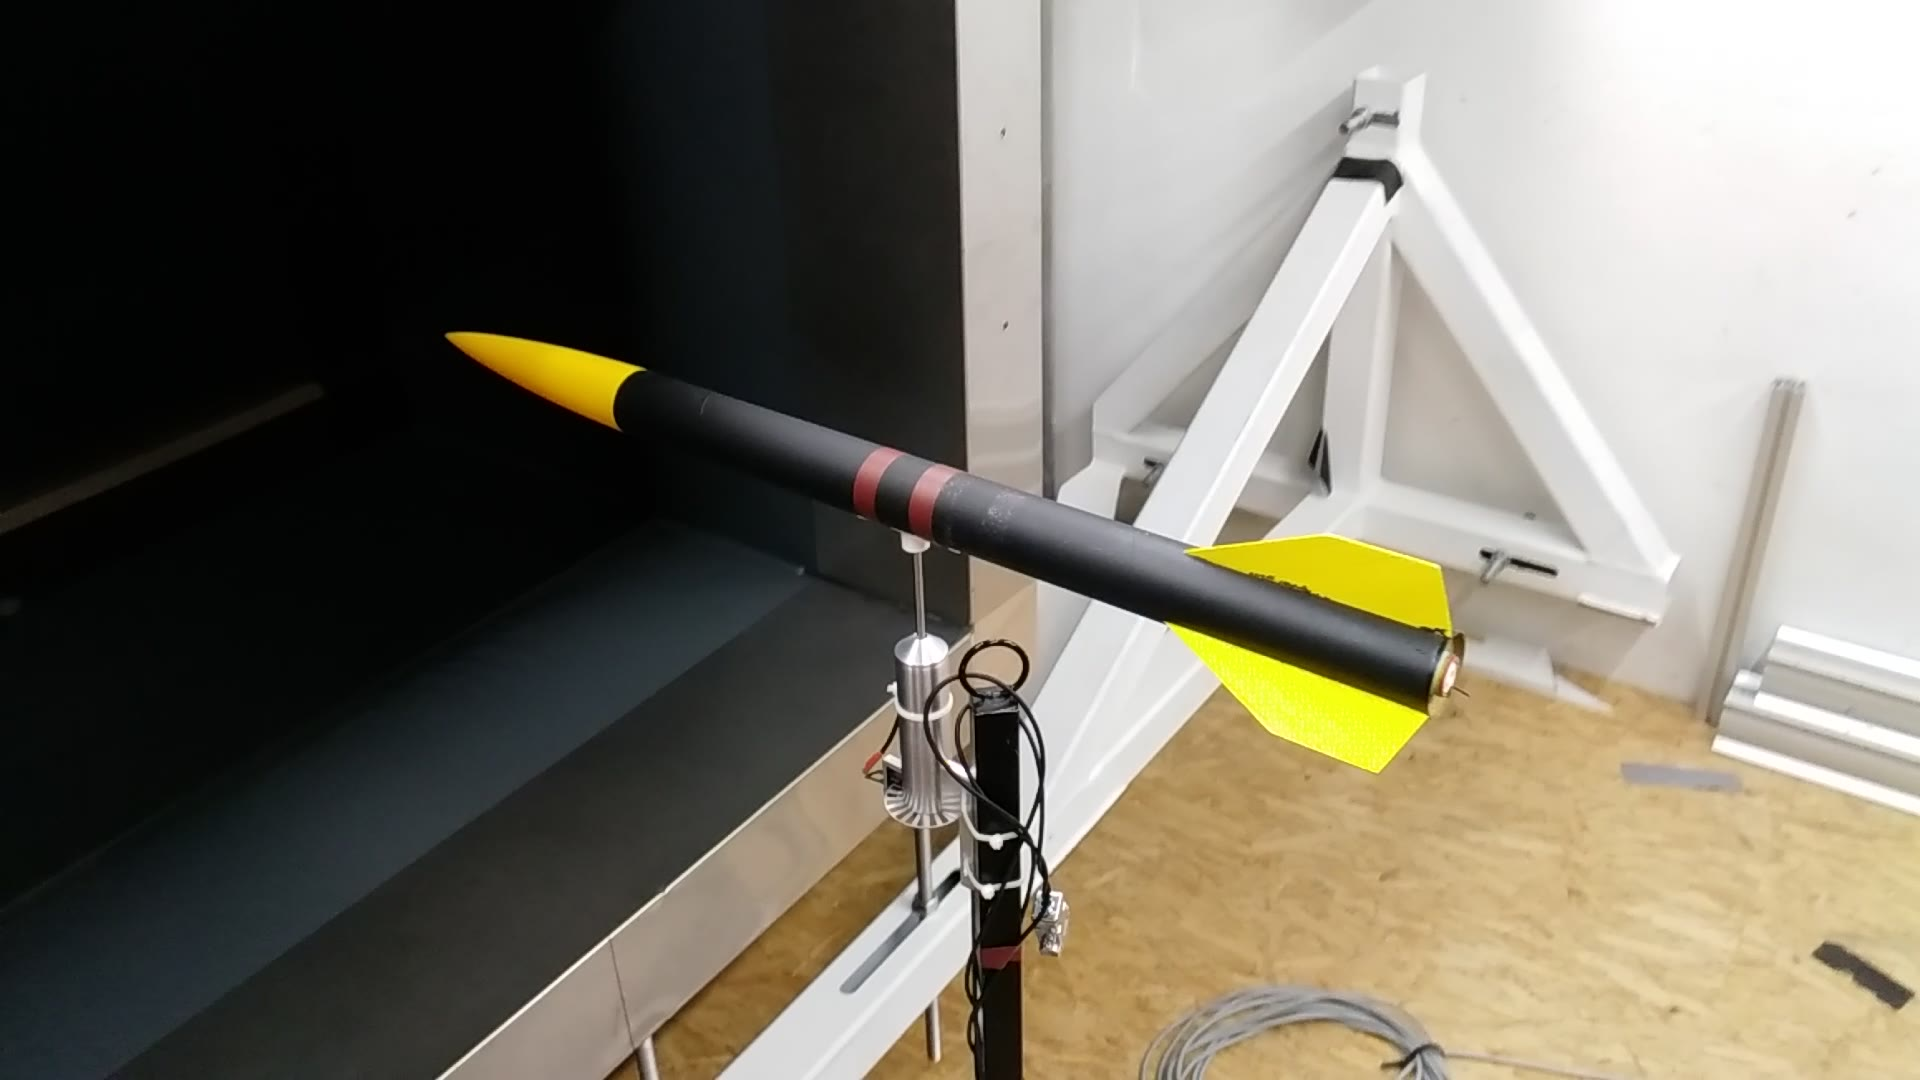
\includegraphics[width=\textwidth]{Bilder/Windkanal-pos1.jpg}
	\subcaption{\texttt{pos1} (Foto: B. Lips)}
	\label{sfig-Windkanal-pos1}
\end{subfigure}\hfill	
\begin{subfigure}[r]{0.49\textwidth}
	\centering
	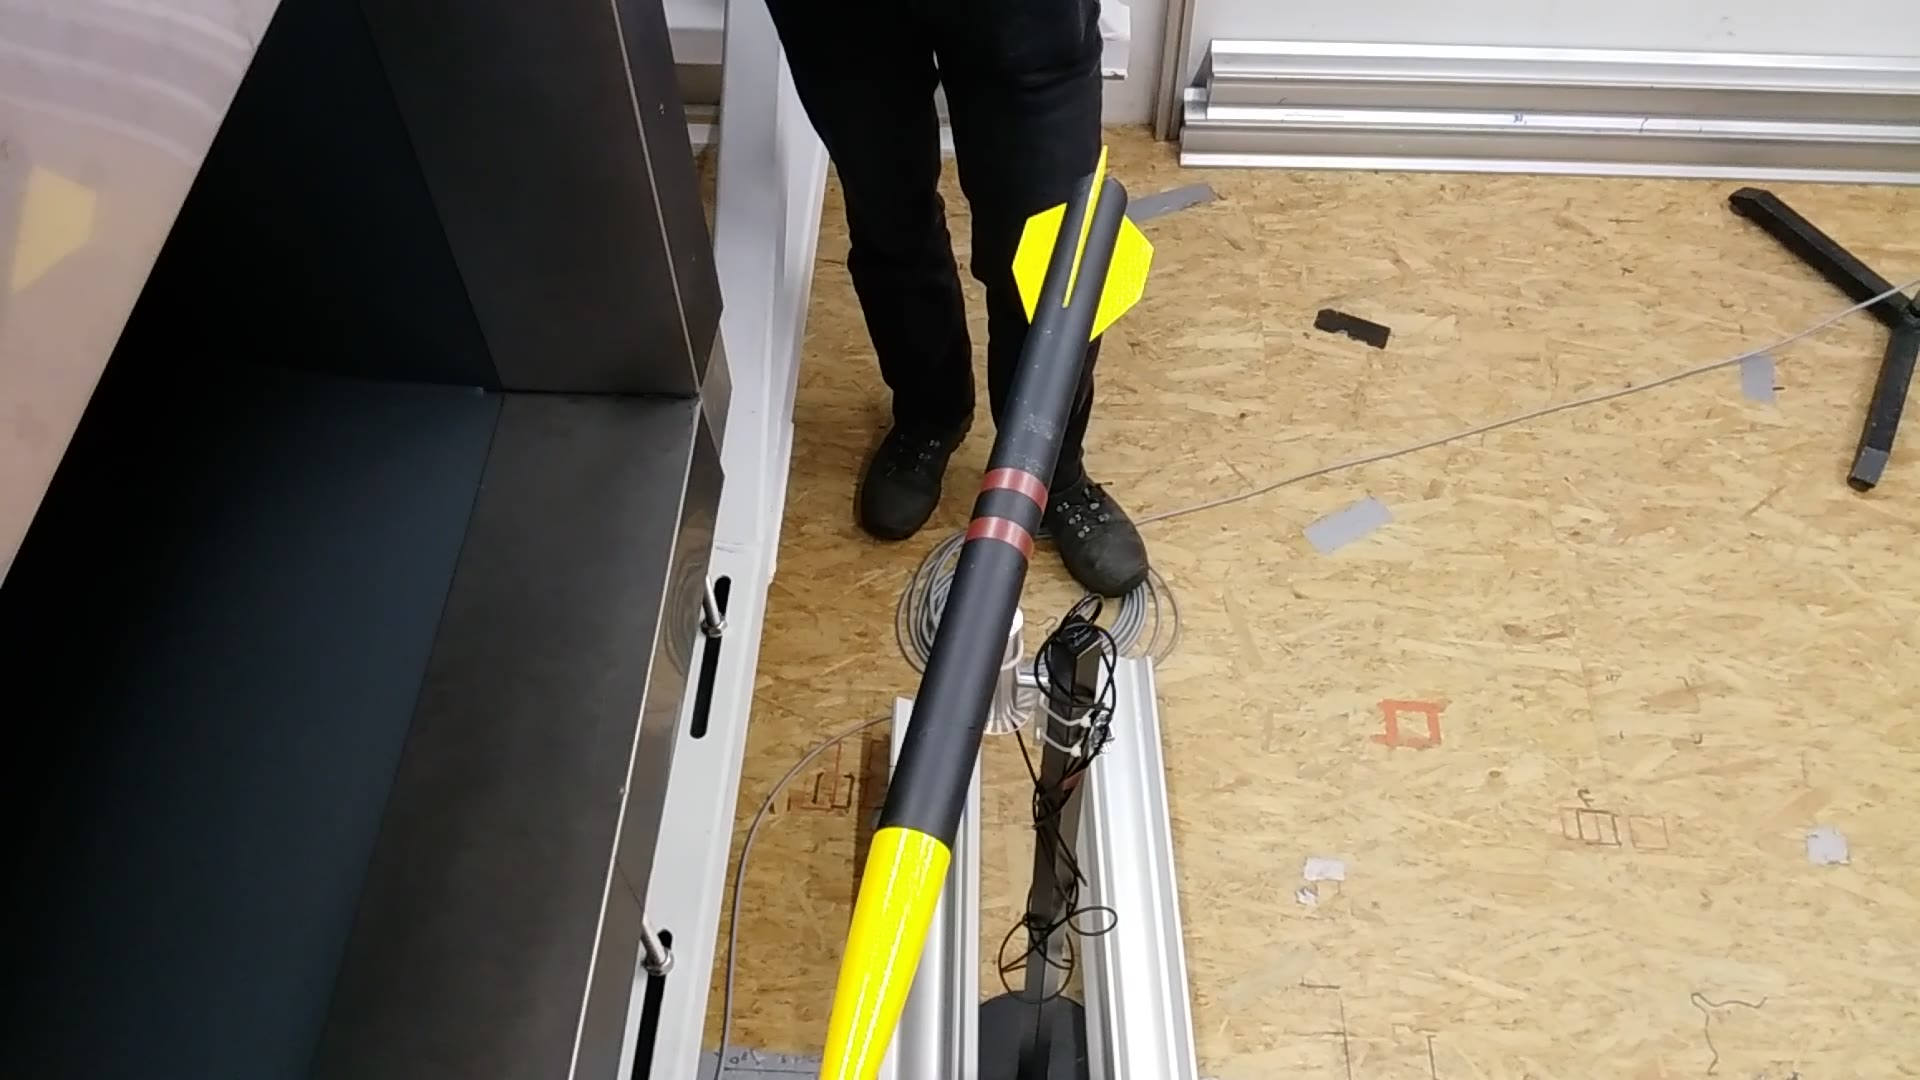
\includegraphics[width=\textwidth]{Bilder/Windkanal-pos2.jpg}
	\subcaption{\texttt{pos2} (Foto: B. Lips)}
	\label{sfig-Windkanal-pos2}
\end{subfigure}
\caption{Die stabilen Positionen von FTV}
\end{figure}

\noindent
Verhalten der Rakete in \texttt{pos2}:

\begin{description}
	\item[Elliptische Spitze] FTV, mit der elliptischen Spitze montiert, verhält sich in \texttt{pos2} verglichen mit den anderen Spitzen sehr stabil. Es ist einfach, die Rakete so zu drehen, dass sie sich in \texttt{pos2} stabilisiert.
	
	\item[Haack Spitze] Bei dieser Raketenspitze ist es schwieriger, die Rakete in \texttt{pos2} zu bringen. Des Weiteren verhält sich die Spitze in \texttt{pos2} längst nicht so stabil. 
	
	\item[Ogive Spitze] Mit der ogiven Raketenspitze ist es noch schwieriger, die Rakete in \texttt{pos2} zu bringen. Befindet sich die Rakete in \texttt{pos2}, so reicht es häufig schon, mit seiner Hand in die Nähe der Rakete zu kommen, um sie wieder in \texttt{pos1} zu bringen.
	
	\item[Konische Spitze] Mit dieser Spitze gibt es \texttt{pos2} nicht. Es gibt keine Position, aus der sich die Rakete quer zum Wind ausrichtet.
	
	\item[Experimentelle Spitze] FTV mit der experimentellen Spitze verhält sich in Bezug auf \texttt{pos2} ähnlich wie die elliptische Spitze. Jedoch macht es hier einen Unterschied, wie die Spitze auf der Rakete steckt. Zeigt die Spitze mit ihrer schmalen Seite zum Luftstrom, pendelt die Rakete in \texttt{pos2} ein wenig hin und her, ohne dass sie sich in einer Position stabilisiert.
	Zeigt die größtmögliche Fläche zum Luftstrom, lässt sich kein Unterschied zur elliptischen Spitze feststellen.	
\end{description}

\noindent
Allen Spitzen ist gemeinsam, dass die Rakete sich erst ab einem Angriffswinkel von über 45 Grad in \texttt{pos2} ausrichtet.

Bei der Stichprobe mit unterschiedlichen Windgeschwindigkeiten konnte im Verhalten der Rakete mit Haack-Spitze kein Unterschied festgestellt werden. Lediglich die Zeit, die vergeht, bis sich die Rakete wieder in eine Position eingependelt, wird mit größerer Windgeschwindigkeit kürzer.

\paragraph{Auswertung}
Das unterschiedliche Verhalten der Raketenspitzen in \texttt{pos2} lässt sich durch die unterschiedlichen Flächen, die zum Luftstrom zeigen, erklären: Die elliptische Spitze ist die bauchigste der Spitzen, somit zeigt bei ihr in \texttt{pos2} die größte Fläche zum Wind. 
Die konische Spitze ist die schlankeste Raketenspitze. Der Luftwiderstand in \texttt{pos2} reicht nicht aus, um ein Kräftegleichgewicht mit dem Luftwiderstand der Leitwerke aufzubauen.
Das Schaukeln der experimentellen Spitze hingegen ist jedoch nur schwierig zu erklären. Denkbar wären zum Beispiel Auswirkungen von durch die Form der Spitze verursachten Turbulenzen.

Das Vorhandensein der stabilen Position \texttt{pos2} erscheint zunächst bedenklich, wenn man sich vorstellt, dass sich die Rakete im Flug nach dieser Position ausrichtet. Dass im Flug einer Rakete mit ausreichender Stabilität in \texttt{pos1} ein so großer Angriffswinkel auftritt, ist jedoch sehr unwahrscheinlich. So gesehen konnte also die Flugstabilität von FTV experimentell bestätigt werden.


\subsection{Flugversuch}

Die Flugstabilität von FTV konnte durch im Flug erneut bestätigt werden, da eine fast senkrechte Flugbahn zu beobachten war. \texttt{pos2} ist im Flug nicht aufgetreten. Für eine genaue Beschreibung des Raketenstarts siehe \ref{ssec-Flugversuch-Luftwiderstand}.


\subsection{Diskussion}

Zunächst liegt ein Widerspruch in der theoretischen Betrachtung der Flugstabilität von FTV und dem Versuch im Windkanal.

An diesem Widerspruch lassen sich die Grenzen der hier beschriebenen Methode zur Berechnung des Druckpunktes feststellen. \texttt{pos2} tritt nur bei großen Angriffswinkeln auf, die theoretische Methode setzt jedoch Angriffswinkel nahe null voraus. So gesehen liegt \texttt{pos2} lediglich außerhalb des Geltungsbereiches der theoretischen Betrachtung. Der Flugversuch und das stabile Verhalten in \texttt{pos1} im Windkanal belegen die vorhergesagte Flugstabilität.



%--------------------------------------------------------------------------------------------------
\section{Fazit und Ausblick}

\paragraph{Fazit}
Es wurde bestätigt, dass die Form der Raketenspitze sowohl Einfluss auf den Luftwiderstand als auch die Flugstabilität hat. Beide Faktoren sind wichtig für die Flugleistung der Rakete.
In Bezug auf die Flughöhe ist die ogive Spitze die optimale, da sie den geringsten Luftwiderstand und ein geringes Gewicht bietet.
In Bezug auf die Flugstabilität hängt die Wahl der optimalen Spitze vom jeweiligen Raketenmodell ab. Eine meist zu geringe Kaliberzahl ist ein gängiges Problem im Modellraketenbau. Die Wahl der Form der Raketenspitze bietet eine Möglichkeit, die Lage des Druckpunktes zu beeinflussen. Der Wechsel der Raketenspitze ist somit ein Werkzeug zum Beheben von Stabilitätsproblemen.

Es kommt im Modellraketenbau jedoch nicht nur auf große Flughöhen an. Auch Faktoren wie die Ästhetik der Rakete spielen eine nicht zu unterschätzende Rolle. So gibt es im Modellraketenbau, wie in fast allen Modellbaudisziplinen, auch originalgetreue Nachbauten von größeren Raketen \cite{om}. Bei solchen Modellen steht die Flughöhe natürlich nicht an erster Stelle.
Somit bleibt die Wahl der besten Raketenspitze persönliche Präferenz. Eine einheitliches Ziel des Modellraketenbaus gibt es nicht. Für Modellraketenbauer, deren Faszination für ihr Hobby vom Reiz der Geschwindigkeit und dem Optimieren der Modelle bis ins letzte Detail geprägt ist, sollten die gewonnenen Erkenntnisse jedoch eine nützliche Wissenserweiterung darstellen.

\paragraph{Ausblick}
In dieser Arbeit wurden Luftwiderstand und Flugstabilität als unabhängige Aspekte behandelt. In Realität hängen diese jedoch eng zusammen, da eine Rakete in Schräglage einen deutlich höheren Luftwiderstand aufweist. Es wäre also wünschenswert beide Aspekte zusammenzuführen und die Stabilität in die Flugsimulation mit einzubeziehen. 
Zusätzlich sollten weitere Parameter als die Spitzenform untersucht werden. Denkbar wären z.B. die Länge der Spitze, die Oberflächenbeschaffenheit etc. 

Unabhängig vom Modellraketenbau können mit den entwickelten Methoden auch viele andere Dinge untersucht werden. Denkbar wären eine Vielzahl an unterschiedlichen Fahrzeugen, wie PKW, LKW, Lokomotiven oder auch Fahrräder mit Verkleidung.



\appendix
%--------------------------------------------------------------------------------------------------
\section{Danksagung an Unterstützer}

Freundlicherweise durften wir für dieses Projekt den Windkanal TWO der Carl von Ossietzky Universität Oldenburg nutzen. Unser Dank geht deshalb an die Universität und in besonderer Weise an unsere Ansprechpartnerin Ingrid Neunaber, die dies ermöglicht hat.

%Bei der folgenden Tabelle handelt es sich um eine Übersicht über die verwendeten Formelzeichen und Abkürzungen. Da dieses Dokument zu lang für die Teilnahme an "Jugend Forscht" gewesen wär, ist sie im finalen Dokument nicht enthalten.

%\section{Formelzeichen}
%
%\begin{table}[H]
%	\begin{tabular}{|r||l|c|}
%		\hline
%		\textbf{Formelzeichen}		& \textbf{Beschreibung}		& \textbf{Einheit}	\\
%		\hline \hline
%		$ A $				& Fläche					& $ \text{m}^2 $	\\
%		$ A_{L} $			& Fläche eines Leitwerks	& $ \text{m}^2 $	\\
%		$ A_{S} $		& Querschnittsfläche der Spitze am ihrem unteren Ende & $\text{m}^2$ \\
%		$ A_{ref} $			& Referenzfläche			& $ \text{m}^2 $	\\
%		$ a $				& Beschleunigung			& $ \text{ms}^{-2} $\\
%		$ a $				& siehe Abb. \ref{Leitwerk-Geometrie-Abb} & m	\\
%		$ b $				& siehe Abb. \ref{Leitwerk-Geometrie-Abb} & m	\\
%		$ C_{n} $			& Auftriebsbeiwert			& --				\\
%		$ C_{n_{L}} $		& Auftriebsbeiwert von einem Leitwerk	& --	\\
%		$ C_{n_{LL}} $		& Auftriebsbeiwert von allen Leitwerken	& --	\\
%		$ C_{n_{S}} $		& Auftriebsbeiwert einer Spitze & --			\\
%		$ C_{W} $			& Widerstandsbeiwert		& --				\\
%		$ d $				& siehe Abb. \ref{Leitwerk-Geometrie-Abb} & m	\\
%		$ D $				& Durchmesser der Rakete	& m					\\
%		$ d' $				& siehe Abb. \ref{Leitwerk-Geometrie-Abb} & m	\\
%		$ F_{G} $			& Gravitationskraft			& N					\\
%		$ F_{Ges} $			& Resultierende Kraft, die auf die Rakete wirkt & N \\
%		$ F_{n} $			& Auftriebskraft			& N					\\
%		$ F_{Schub} $		& Schubkraft des Raketenmotors & N 				\\
%		$ F_{W} $			& Aerodynamische Widerstandskraft & N			\\
%		$ g $				& Ortsfaktor				& $ \text{ms}^{-2} $\\
%		$ K $				& Korrekturfaktor			& --				\\
%		\texttt{Kal}		& Kaliberzahl				& m					\\
%		$ l $				& siehe Abb. \ref{Leitwerk-Geometrie-Abb} & m	\\
%		$ L_{K} $			& Länge des Körperrohrs		& m					\\
%		$ L_{S} $			& Länge der Raketenspitzen	& m					\\
%		$ m $				& Masse						& kg 				\\
%		$ M_{n} $			& Drehmoment um $ X_{0} $	& Nm				\\
%%		$ n $				& Anzahl der Leitwerke		& --				\\
%		$ R $				& Radius der Rakete			& m					\\
%		$ r(x) $			& Radius einer Raketenspitze als Funktion ihrer Länge & m \\
%		$ s $				& Strecke					& m					\\
%		$ s $				& siehe Abb. \ref{Leitwerk-Geometrie-Abb} & m	\\
%		$ t $				& Zeit						& s					\\
%		$ v $				& Geschwindigkeit			& $ \text{ms}^{-1}$	\\
%		$ V_{S} $			& Volumen der Spitze		& $ \text{m}^3 $	\\
%		$ x $				& Position eines Punktes auf der Mittelachse der Raketenspitze & m \\
%		$ X_{0} $			& Punkt am unteren Ende der Rakete & --			\\
%		$ x_{DP} $			& Strecke von Unterkante der Rakete bis DP & m				\\
%		$ x_{LL} $			& Strecke von Unterkante der Rakete bis DP eines Leitwerkes& m				\\
%		$ x_{S} $			& Strecke von Unterkante der Rakete bis DP der Spitze & m	\\
%		$ x_{SP} $			& Strecke von Unterkante der Rakete bis SP & m				\\
%		$ \alpha $			& Angriffswinkel			& --				\\
%		$ \gamma $			& siehe Abb. \ref{Leitwerk-Geometrie-Abb} & --	\\
%		$ \Gamma $			& siehe Abb. \ref{Leitwerk-Geometrie-Abb} & --	\\
%		$ \rho $			& Luftdichte				& $ \text{kgm}^{-3}$\\
%		$ \rho_{t} $		& Radius des Kreisabschnittes einer ogiven Spitze & m \\
%%		\hline
%%		DP					& Druckpunkt				& n/A				\\
%%		FTV					& Flight Test Vehicle	& n/A				\\
%%		SP					& Schwerpunkt				& n/A				\\
%		\hline
%		
%	\end{tabular}
%	
%\end{table}



\newpage
\begin{thebibliography}{99}
	\addcontentsline{toc}{section}{Literatur} 
	\bibitem{brock}
	Brockhaus: ballistische Rakete. \\
	\url{http://brockhaus.de/ecs/enzy/article/ballistische-rakete} (07.02.2018)
	
	\bibitem{dlr}
	Deutsches Zentrum für Luft- und Raumfahrt (2007): Windkanal. Wie man Fahrzeuge noch windschlüpfriger macht.\\
	\url{http://www.dlr.de/schoollab/Portaldata/24/Resources/dokumente/hb/windkanal.pdf} (09.01.2019; 10:54)
	
	\bibitem{elv}
	ELV Elektronik. Datenblatt Digitalmultimeter UT~70~A.
	\url{https://files.elv.com/service/manuals_hw/71714_UT70A_UM.pdf} (11.01.2019; 20:37)
	
	\bibitem{AbR}
	Fachlabor Raumfahrttechnik: Versuch "`Aerodynamisch-ballistische Rakete"'. Technische Universität Braunschweig.
	\url{https://www.er-ig.de/cms/uploads/Skript_Raketenstart.pdf} (09.01.2019;~10:56)
	
	\bibitem{hw}
	Hucho, Wolf-Heinrich (2002): Aerodynamik der stumpfen Körper. Physikalische Grundlagen und Anwendungen in der Praxis. 2. Auflage. Vieweg + Teuber Verlag. Wiesbaden.
	
	\bibitem{klima}
	Klima: Raketenmotorfibel. \\
	\url{http://www.neu.raketenmodellbau-klima.de/Download_Dateien/Motorflyer_DINA4.pdf} (09.01.2019;~10:56)
	
	\bibitem{dl}
	Lancelle, Daniel (2008): Entwurf eines Autopiloten für Experimentalraketen. 1. überarbeitete Veröffentlichung.
	Technische Universität Braunschweig.
	\url{https://www.raketenmodellbau.org/repository/archive/126750?view=true} (09.01.2019;~10:57)
	
	\bibitem{lp}
	Leifi Physik: Luftreibung.\\ \url{https://www.leifiphysik.de/mechanik/reibung-und-fortbewegung/luftreibung} (09.01.2019;~10:58)
	
	\bibitem{fs}
	Meyer, L./ Gramm, A./ Benecke, K. und weitere (2012): Das große Tafelwerk. interaktiv 2.0. Niedersachsen. Berlin. 
	
	\bibitem{hm}
	Mielke, Heinz (1967): Meyers Taschenlexikon Raketentechnik Raumfahrt. Leipzig. 
	
	\bibitem{om}
	Missbach, Oliver (2001): Fliegende Modellraketen selbst gebaut 2.Auflage. Edition Countdown. München. 
	
	\bibitem{sn}
	Niskanen, Sampo (2009): Development of an Open Source model rocket simulation software. Helsinki University of Technology. \url{http://openrocket.sourceforge.net/thesis.pdf} (09.01.2019;~10:59)
	
	\bibitem{pce}
	PCE Instruments. Datenblatt PCE-FM50. \\
	\url{http://static.mercateo.com/e5/c5859a1fca4548a3a8d0e41d29182954/pdf/kraftmessgeraet-pce-fm50.pdf} (11.01.2019;~20:30)
	
	\bibitem{ew}
	Willerding, Eugen (2018): Die mathematische Theorie ballistischer Kurven.\\ \url{https://www.eugen-willerding.de/app/download/5785857957/ballistik.pdf} (09.01.2019;~10:59)
\end{thebibliography}

\end{document}
